\documentclass[12pt]{article}
\usepackage[a4paper,margin=1in,footskip=0.25in]{geometry} % set margins
\usepackage[portuguese]{babel}
\usepackage[utf8]{inputenc}
\usepackage[hidelinks]{hyperref} 
\usepackage{amsmath}
\usepackage{amssymb}
\usepackage{amsthm}
\usepackage{graphicx}    % needed for include graphics
\usepackage[space]{grffile}
\usepackage{subfigure}   % add subfigures
\usepackage{indentfirst}
\usepackage{float}       % needed for [H] figure placement option
\usepackage{setspace}    % needed for doublespacing
\usepackage{tikz}
\usepackage{algpseudocode}
\usepackage{listings}
\usepackage{xcolor}

\definecolor{mGreen}{rgb}{0,0.6,0}
\definecolor{mGray}{rgb}{0.5,0.5,0.5}
\definecolor{mPurple}{rgb}{0.58,0,0.82}
\definecolor{backgroundColour}{rgb}{0.95,0.95,0.92}

\lstdefinestyle{CStyle}{
    backgroundcolor=\color{backgroundColour},   
    commentstyle=\color{mGreen},
    keywordstyle=\color{magenta},
    numberstyle=\tiny\color{mGray},
    stringstyle=\color{mPurple},
    basicstyle=\footnotesize,
    breakatwhitespace=false,         
    breaklines=true,                 
    captionpos=b,                    
    keepspaces=true,                 
    numbers=left,                    
    numbersep=5pt,                  
    showspaces=false,                
    showstringspaces=false,
    showtabs=false,                  
    tabsize=2,
    language=C
}

% Macros
\renewcommand{\familydefault}{\sfdefault} % sans-serif
\newcommand{\lowtext}[1]{$_{\text{#1}}$}
\newcommand{\code}[1]{\texttt{#1}}

% Adds ./img/ to the path of figures
\graphicspath{{img/}}

\title{Relatório EP2 - MAC0219}
\author{Bruno Sesso, Gustavo Estrela de Matos}

\begin{document}
% Espaçamento duplo 
\doublespacing
\begin{titlepage}
    \vfill
    \begin{center}
        \vspace{0.5\textheight}
        \noindent
        Instituto de Matemática e Estatística \\
        EP1 - MAC0219 \\
        \vfill
        \noindent
        {\Large Implementação de Algoritmos de Criptografia e Codificação
                Paralelos Usando CUDA} \\
        \bigskip
        \bigskip
        \begin{tabular}{ll}
            {\bf Professor:} & {Alfredo Goldman} \\
            {\bf Alunos:}    & {Bruno Sesso} \\
                             & {Gustavo Estrela de Matos} \\
        \end{tabular} \\
        \vspace{\fill}
       \bigskip
        São Paulo, \today \\
       \bigskip
    \end{center}
\end{titlepage}

\pagebreak
\tableofcontents
\pagebreak


%%%%%%%%%%%%%%%%%%%%% INTRODUÇÃO %%%%%%%%%%%%%%%%%%%%%%%%%%%%%%%%%%%%%
\newpage
\section{Introdução}
Este trabalho tem como objetivo a paralelização e análise de desempenho
de algoritmos de criptografia e codificação para serem rodados em GPUs.
O código desenvolvido utilizará a biblioteca \emph{Compute Unified 
Device Architecture} (CUDA), e portanto será compatível apenas com GPUs 
NVIDIA.

Pensando na arquitetura \emph{multiple instruction single data} (MISD), 
escolhemos três algoritmos em que os dados não possuem grandes 
dependência entre si, e portanto podem ser separados mais facilmente 
para serem processados em paralelo. Os três algoritmos escolhidos foram:
\begin{itemize}
    \item{\textbf{Base64}}: um algoritmo de codificação;
    \item{\textbf{Rot13}}: também um algoritmo de codificação;
    \item{\textbf{Vigenere}}: um algoritmo de cifração.
\end{itemize}
        
Para analisar a paralelização dos algoritmos a nossa principal métrica
foi o tempo de execução ao processar arquivos de texto. Os três 
algoritmos escolhidos não tem grandes dependências ao conteúdo lido, 
portanto escolhemos arbitrariamente uma versão em texto puro da Bíblia
para medir tempos de execução. Para garantir significância estatística
utilizamos o programa \emph{perf}, que nos permite apresentar resultados
médios de rodadas do algoritmo.

% todo: falar onde a gente rodou as paradas. Qual as configs da placa?
O computador utilizado para realizar os testes foi o \emph{terra} 
(terra.eclipse.ime.usp.br), que conta com uma GPU GeForce GTX 750,
rodando CUDA 8.0, e 4 Multiprocessors de 128 CUDA cores cada. 


%%%%%%%%%%%%%%%%%%%%% ALGORITMOS %%%%%%%%%%%%%%%%%%%%%%%%%%%%%%%%%%%%%%%
% Aqui a gente explica os algoritmos que a gente escolheu e mostra
% como a versão sequencial deles funciona
\newpage
\section{Algoritmos Escolhidos}
\subsection{Base64}
\emph{Base64} é um algoritmo de codificação principalmente utilizado 
para transferência de dados na internet que transforma cada 6 bits 
da entrada em um caractere de texto da codificação. A implementação que 
escolhemos faz essa operação em blocos, e transforma cada três
caracteres da entrada ($3 * 8$ bits) em quatro caracteres de texto da
codificação ($4 * 6$ bits).

\subsection{Rot13}
\emph{Rot13} é um algoritmo bastante simples em que cada letra é
trocada por uma 13 índices a frente. Por exemplo: a letra "a" é
substituída pela letra "n", a letra "b" por "o" e assim por diante.
Para implementar uma versão que possa ser rodada em uma GPU separamos
a simples operação de somar 13 para cada caractere e a passamos como
kernel. 

\subsection{Vigenere}
\emph{Vigenere} é um algoritmo de criptografia, diferente dos últimos 
dois algoritmos de codificação citados. A diferença de um algoritmo de
criptografia para um de codificação é que para se obter o texto 
original, esse algoritmo deve usar uma chave específica. O algoritmo
Vigenere é antigo e suas primeiras implementações foram feitas em 
objetos mecânicos, datados em meados do século 1400.

O algoritmo Vigenere original encripta somente caracteres do alfabeto
siciliano e, como isto cria uma dependência entre os dados do texto
(o que complica a estrutura do código paralelo), resolvemos implementar 
uma versão do código que também codifica caracteres que são dígitos 
e espaços.


%%%%%%%%%%%%%%%%%%%%% ARQUITETURA NVIDIA %%%%%%%%%%%%%%%%%%%%%%%%%%%%%%%
\newpage
\section{Arquitetura CUDA}
Antes de mostrarmos nossos experimentos precisamos entender um pouco da
arquitetura CUDA. Os principais conceitos que usamos durante esse 
trabalho foram de blocks, threads, streaming multiprocessors (SM), warps
e cuda cores, e entender como eles se relacionam é fundamental para
produzir um código que faça o melhor uso possível da GPU. Primeiro,
devemos explicitar que o conceito de thread e bloco são divisões do 
trabalho que são especificadas pela própria aplicação, enquanto que
Streaming Multiprocessors e cuda cores são características físicas da
placa de vídeo. 

Quando nossa aplicação "lança" um código para ser rodado na GPU, i.e um 
kernel, cada block é associado a um SM e as threads de cada bloco
são agrupadas em conjuntos de 32 threads, chamado de warp. O SM, por sua
vez, escalona as warps dos blocks para serem processados. Chamamos uma
warp escalonada de residente.

Se quisermos maximizar o desempenho do um programa cuda paralelo devemos
nos atentar a dois pontos principais: balanceamento de carga e 
ocupação. O primeiro ponto não é uma preocupação real nesse trabalho, 
porque o processamento dado ao texto nos três programas escolhidos é bem
balanceado por natureza e existem poucos desvios no código, isto é, 
o processamento é idêntico na maior parte da entrada. Por outro lado, a
ocupação dos recursos da GPU é um assunto complexo que será rasamente
abordado nesse trabalho.

A ocupação dos recursos de um SM é a razão entre o número de warps sendo
processadas e o número máximo de warps que um SM pode processar. É 
difícil determinar o primeiro valor citado, porém podemos ao menos 
garantir que estamos criando um número de threads que pode atingir o 
número máximo de warps que o SM é capaz de processar. 

A placa de vídeo que utilizamos, uma GTX 750 possui 4 Streaming 
Multiprocessors, que possuem um limite de 64 warps cada, e também um 
limite de 1024 threads por bloco. Como cada warp dessa arquitetura
possui 32 threads, temos que para ocupar um SM precisamos criar pelo
menos 2048 (64 * 32) threads, e como cada bloco pode ter no máximo 1024
threads, precisamos também de 2 blocos. É importante notar também que a
GPU processa, no melhor caso, warps inteiras, portanto é ideal que 
usemos blocos com tamanhos múltiplos do tamanho do warp, garantindo que 
não haverá warps que não utilizam todo poder do SM.

Na próxima seção apresentamos os experimentos feitos e ao final 
concluímos com a melhor divisão de trabalho que pudemos observar.


%%%%%%%%%%%%%%%%%%%%% EXPERIMENTO %%%%%%%%%%%%%%%%%%%%%%%%%%%%%%%%%%%%%%
% Aqui agente explica como fizemos os testes nossa metodologia, etc.. 
% coisas que são compartilhadas pelos experimentos de todos os 
% algoritmos
\newpage
\section{Os experimentos}
Para cada um dos algoritmos analisados realizamos uma série de testes. 
Como queríamos analisar o desempenho dos algoritmos em relação ao 
tamanho de entrada, utilizamos uma versão em texto da bíblia em
diversos tamanhos. O texto da bíblia que usamos tem 4452070 caracteres.
A partir desse texto, criamos arquivos com o mesmo texto repetido 1, 2,
4 e 8 vezes. Isto é, criamos arquivos de testes que crescem 
exponencialmente na quantidade de caracteres.

Nosso primeiro teste verifica o tempo necessário para que a 
implementação sequencial do algoritmo em questão leva para processar os
arquivos de testes, as bíblias.

Para o algoritmo implementado para rodar na GPU, verificamos não
somente o tempo em relação ao tamanho dos arquivos de entrada como
também em relação ao número de threads por bloco. Como no caso ideal o
número de threads deve ser múltiplo de 32, verificamos para todos os
múltiplos de 32 a 1024 (máximo de threads por bloco).
%todo: explicar porque deve ser múltiplo de 32

Por fim, verificaremos também o tempo levado para se fazer a leitura dos
arquivos. A leitura é feita igualmente para ambas as implementações de
cada algoritmo de encriptação, portanto queremos verificar se o tempo
levado para a execução de cada é relacionado às operações de leitura.


%%%%%%%%%%%%%%%%%%%%% DISCUSSÃO DOS RESULTADOS %%%%%%%%%%%%%%%%%%%%%%%%%
\newpage
\section{Discussão dos Resultados}
Nessa seção apresentamos os resultados obtidos em cada um dos três 
algoritmos paralelizados. Como os três algoritmos fazem trabalhos 
parecidos, de substituição de caracteres, os resultados e as conclusões tomadas. Para evitar redundância, vamos 
apresentar primeiro, com mais detalhe, os resultados do algoritmo Rot13
e depois, de maneira menos detalhada, os resultados de Base64 e 
Vigenere.

\subsection{Rot13}

Primeiramente analisemos o tempo levado da implementação sequencial.
Sabemos que o programa realiza uma operação igual para cada caractere.
Portanto esperamos que o tempo de um algoritmo sequencial seja linear
para o tamanho do array de caracteres. Observamos tal comportamento no
seguinte gráfico:

\begin{figure}[H]
    \makebox[\textwidth][c]{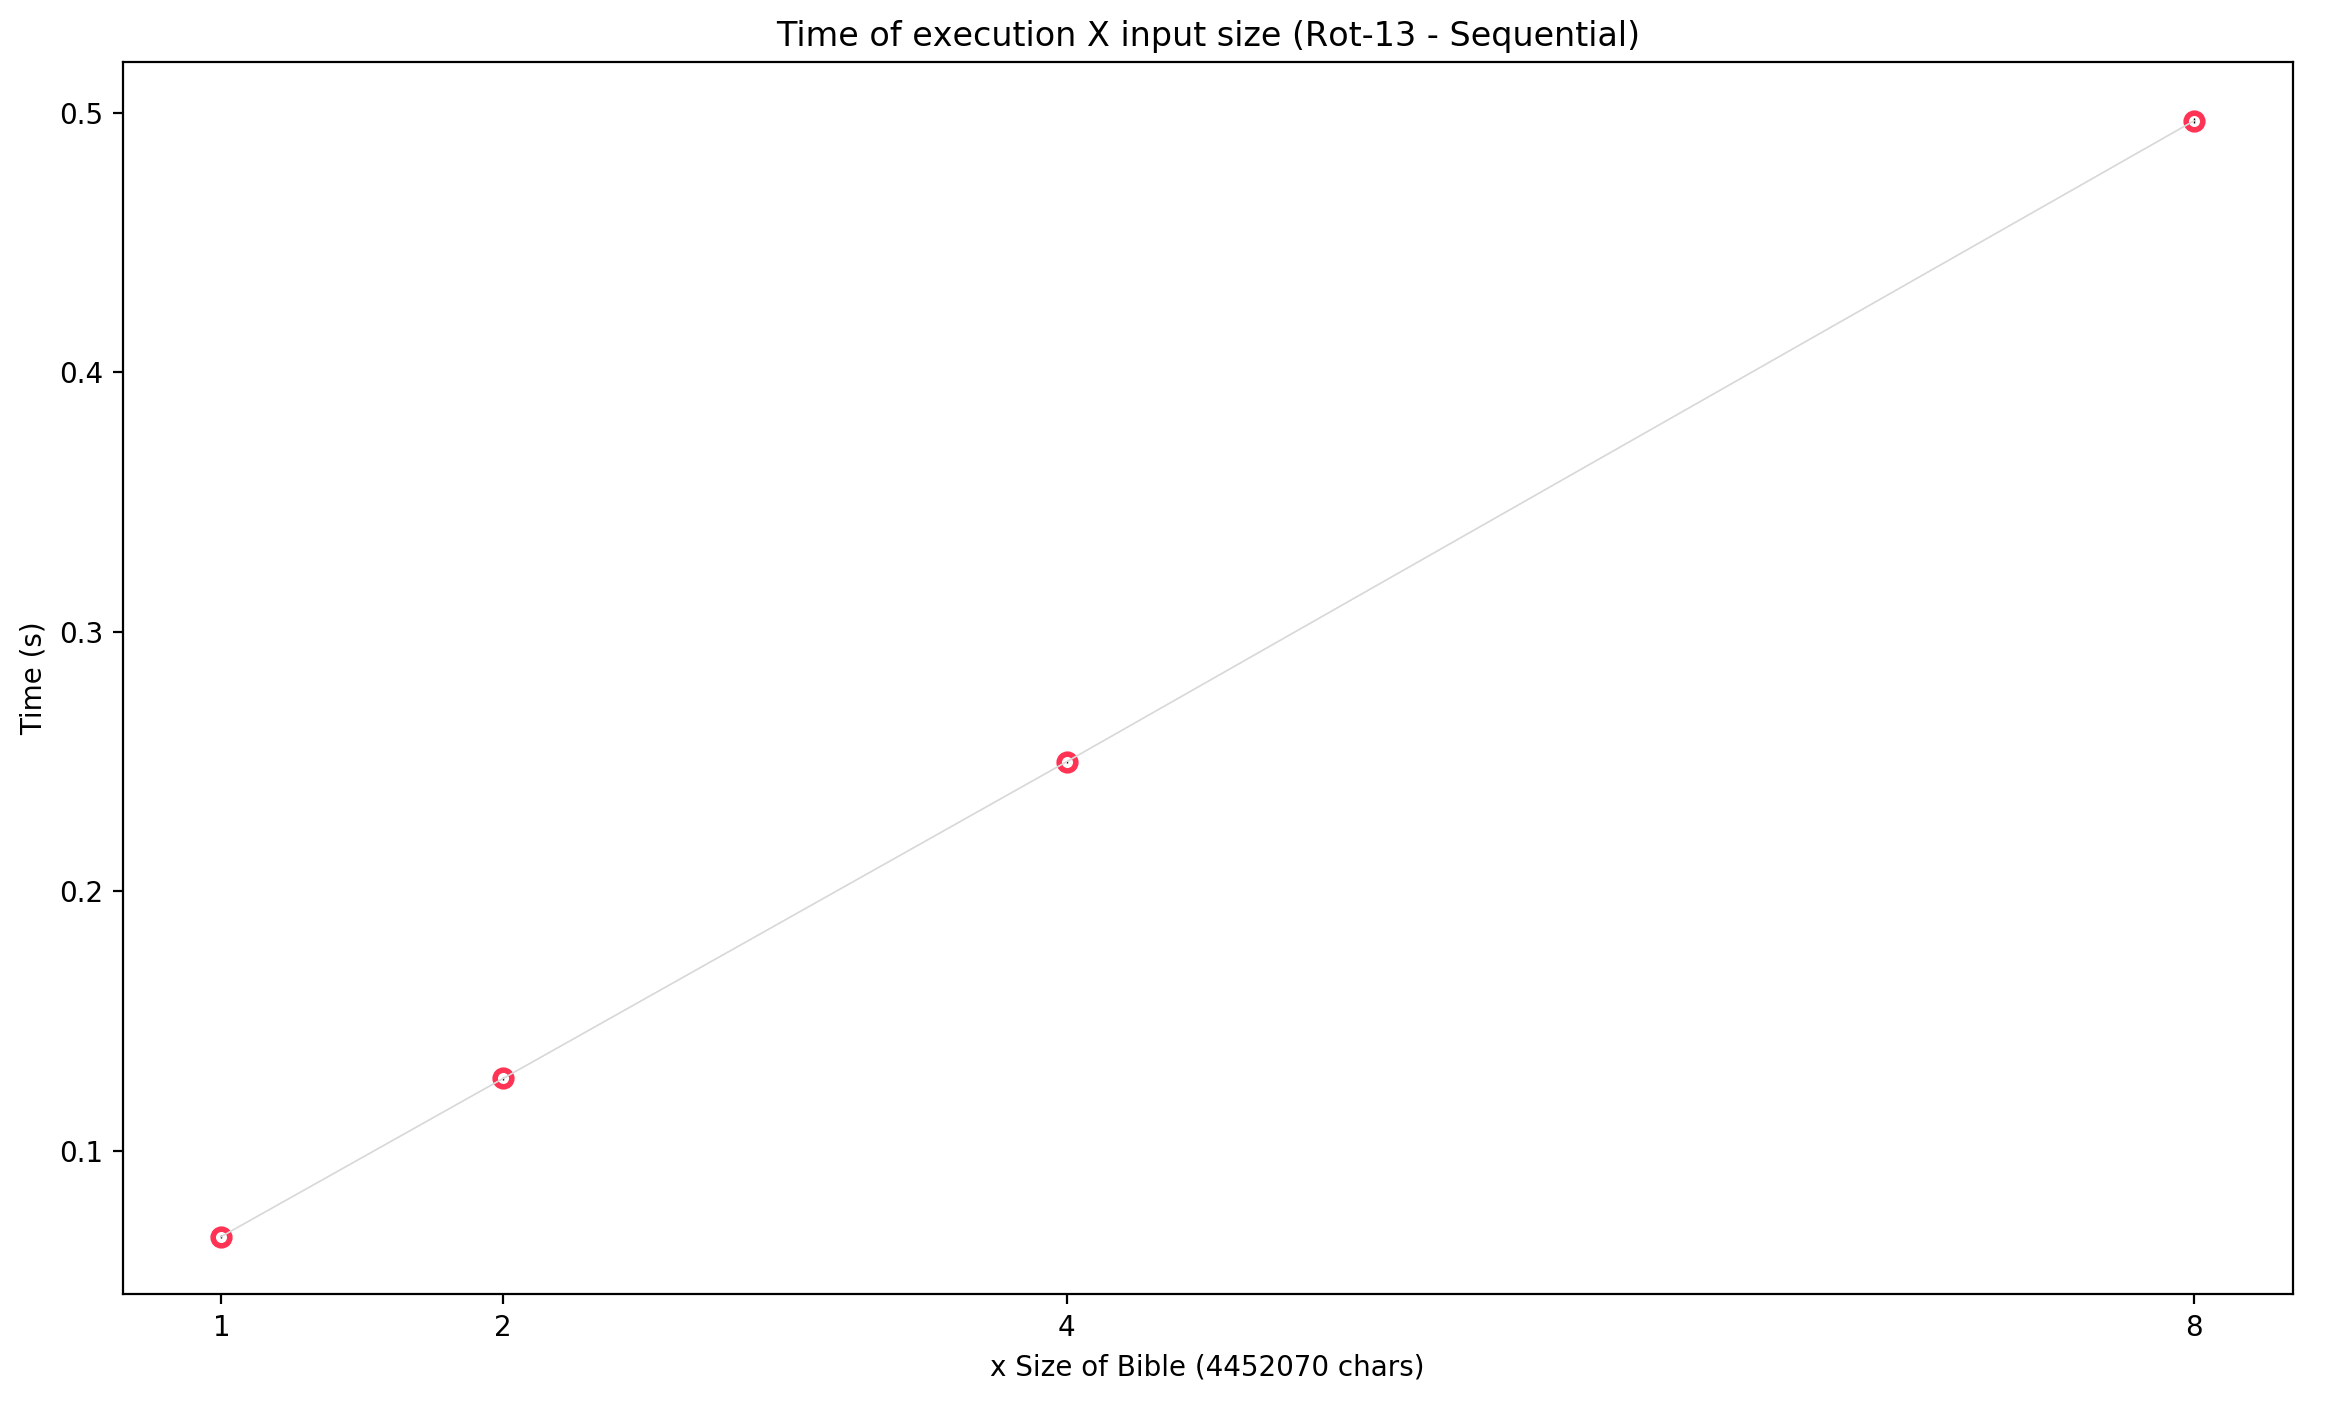
\includegraphics[scale=.65]{img/rot13_seqXpar/timeXsize_Rot-13 - Sequential.png}}
    \caption{Tempo de execução do algoritmo Rot13 sequencial.}
\end{figure}

Apesar de 8 vezes o tamanho da bíblia (35.616.560 caracteres) ser um
número bastante grande, até mesmo o algoritmo sequencial o realiza em
apenas meio segundo. Esperamos que a implementação paralela, realize os
cálculos pelo menos mais rápido que a implementação sequencial:

\begin{figure}[H]
    \makebox[\textwidth][c]{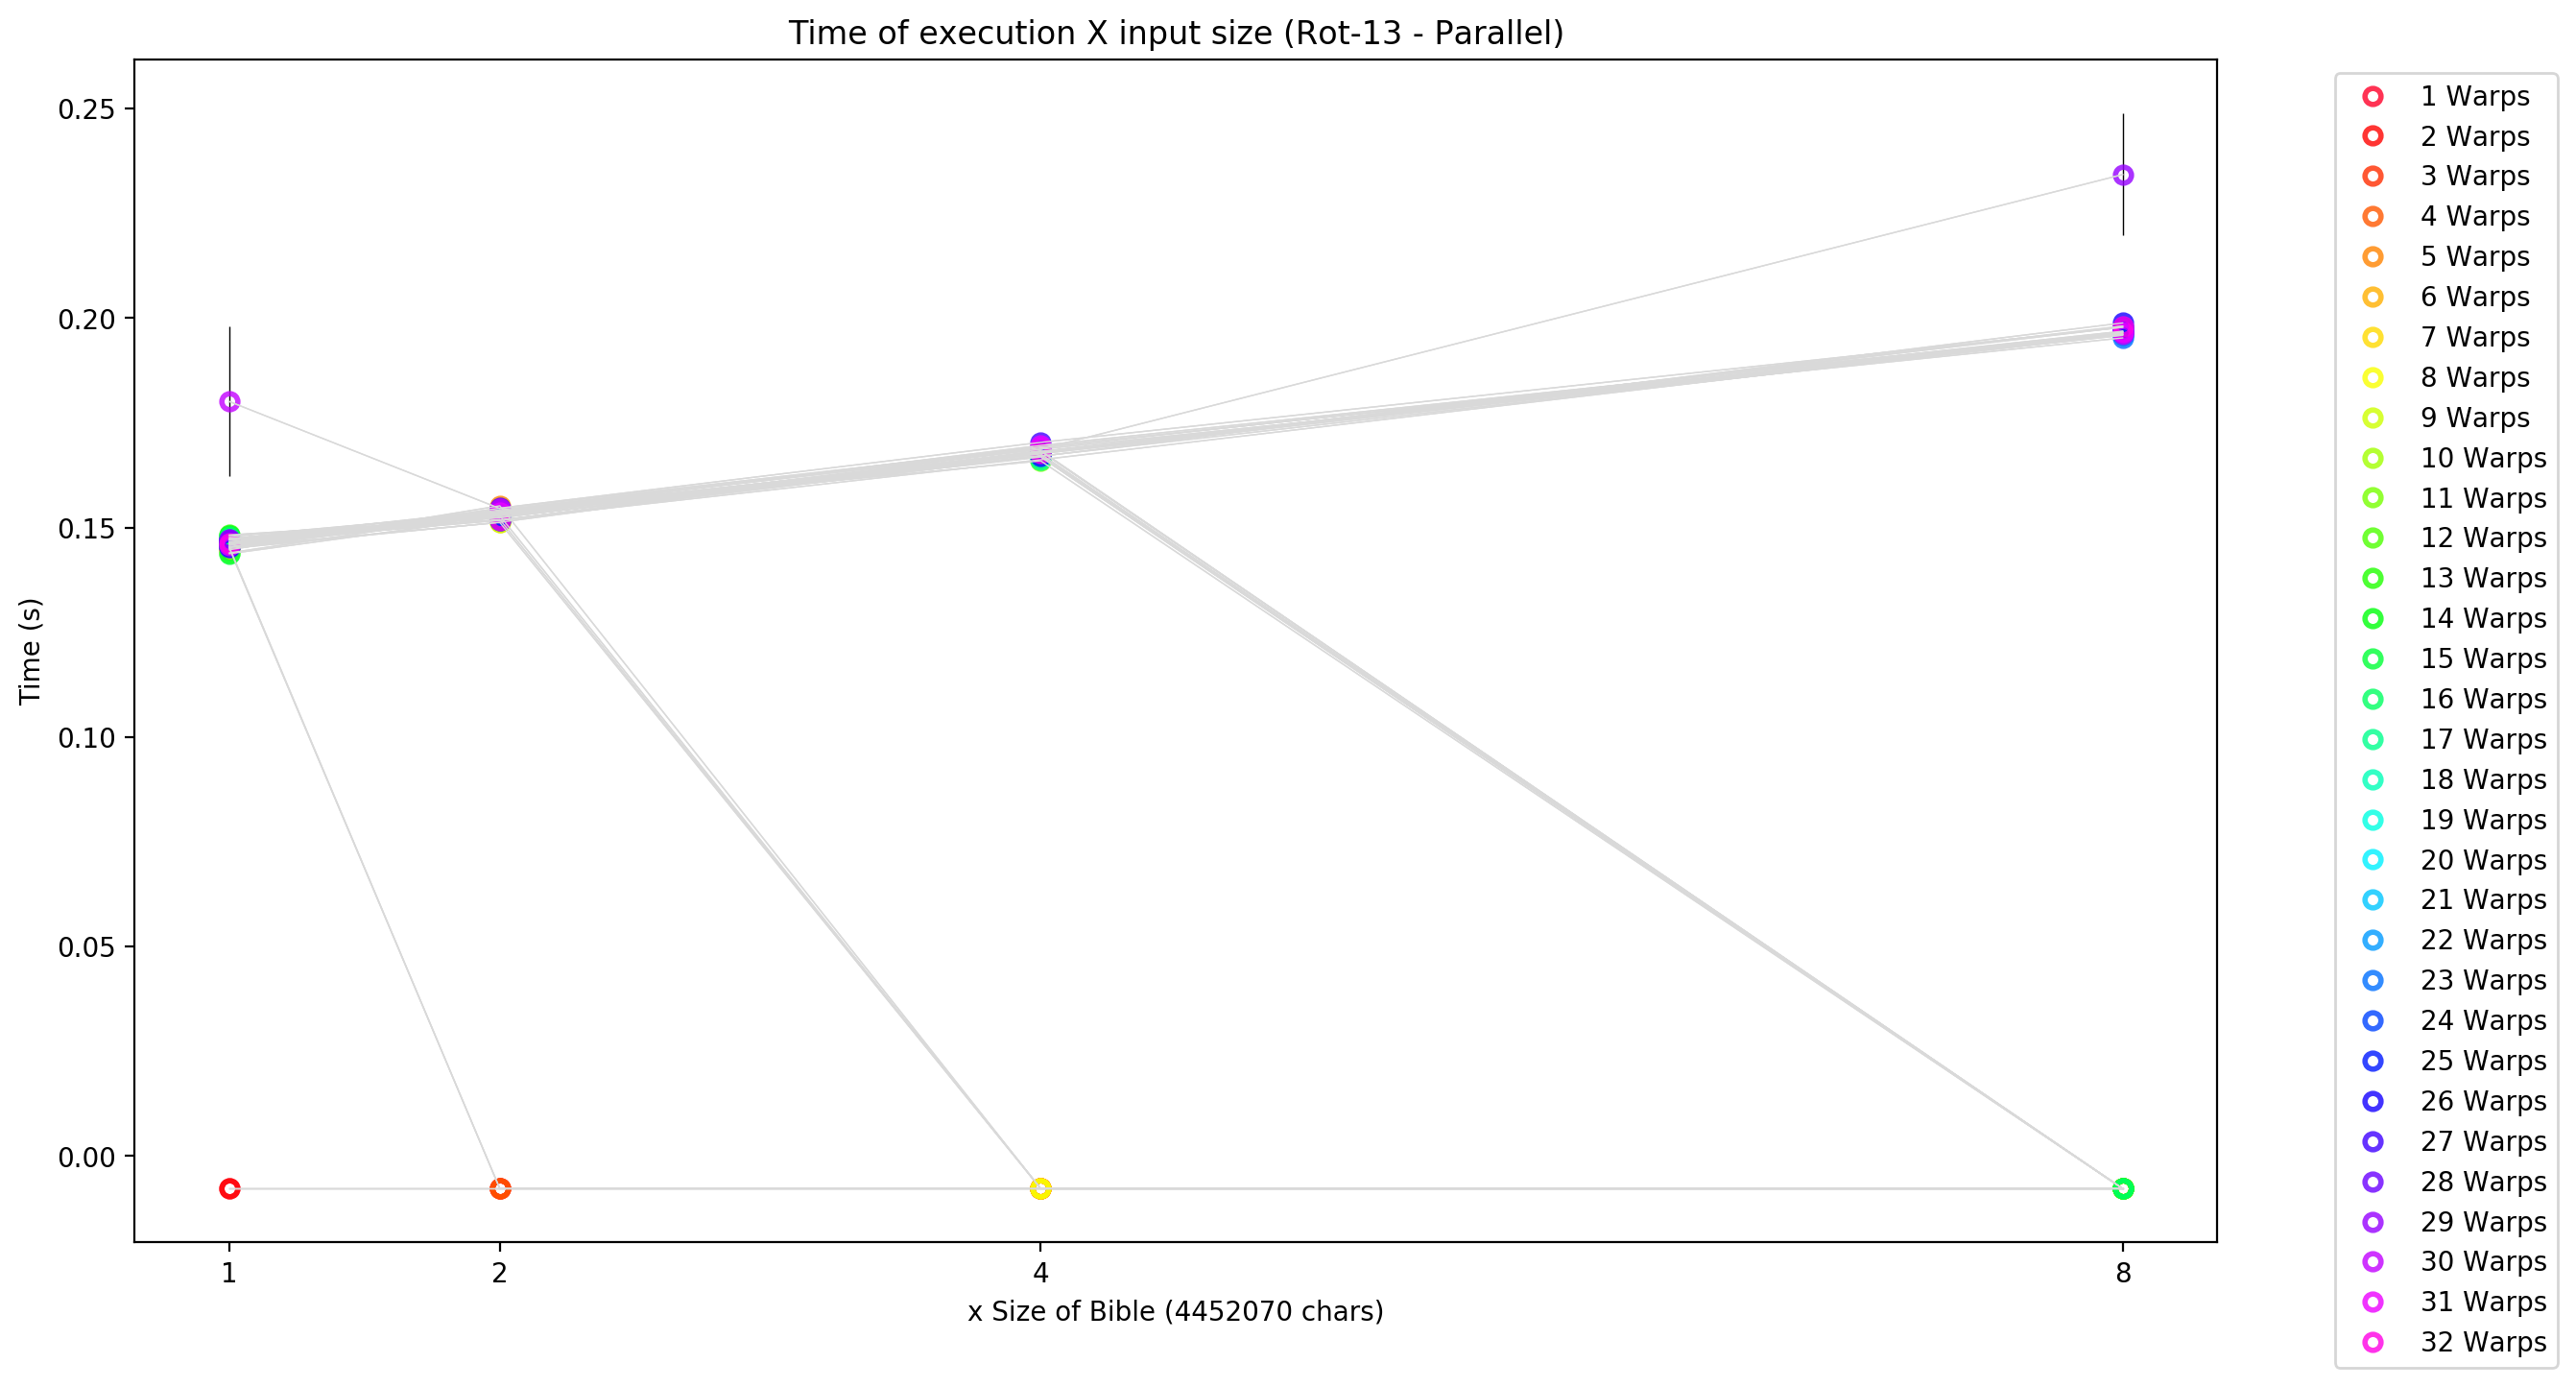
\includegraphics[scale=.55]{img/rot13_seqXpar/timeXsize_Rot-13 - Parallel.png}}
    \caption{Tempo de execução do algoritmo Rot13 paralelo variando o
    tamanho de entrada.}
\end{figure}

Como esse gráfico possui mais informações analisemos-o com mais cuidado.
O eixo Y representa o tempo levado para o algoritmo ser executado.
O eixo X representa o tamanho dos arquivos de entrada. Em cada execução
do programa, utilizamos um valor de threads por bloco. 1 warp 
representa 32 threads. Para cada valor de 1 a 32 warps, uma cor é
utilizada no gráfico. Além disso, para algumas combinações de número de
threads e de tamanho de entrada, há falha ao passar tais argumentos
para a GPU. Nesses casos representamos o tempo do algoritmo por um valor
um pouco abaixo de 0 no gráfico. Comecemos a analisar o gráfico.

Para cores roxas e mais azuladas, notamos que elas seguem o mesmo padrão
linear de aproximadamente 0,15s a 0,18s. Há valores aonde erros
ocorrem, pois o número de blocos necessários para a combinação
ultrapassaria o número máximo de blocos da GPU. Por exemplo para 1 warp
(32 threads) e tamanho de entrada 1 Bíblia (4.452.070 caracteres) há a
necessidade de 139.128 blocos, que ultrapassa o número máximo de blocos
da GPU (65535). Ou seja, quando aumentamos o tamanho do arquivo de
entrada, algum dos valores de número de warps por bloco passam a ser
inválidos, pois iriam requirir blocos demais. É interessante notar que
para os valores adequados de warps por blocos o tempo de execução do
programa é o mesmo:

\begin{figure}[H]
    \makebox[\textwidth][c]{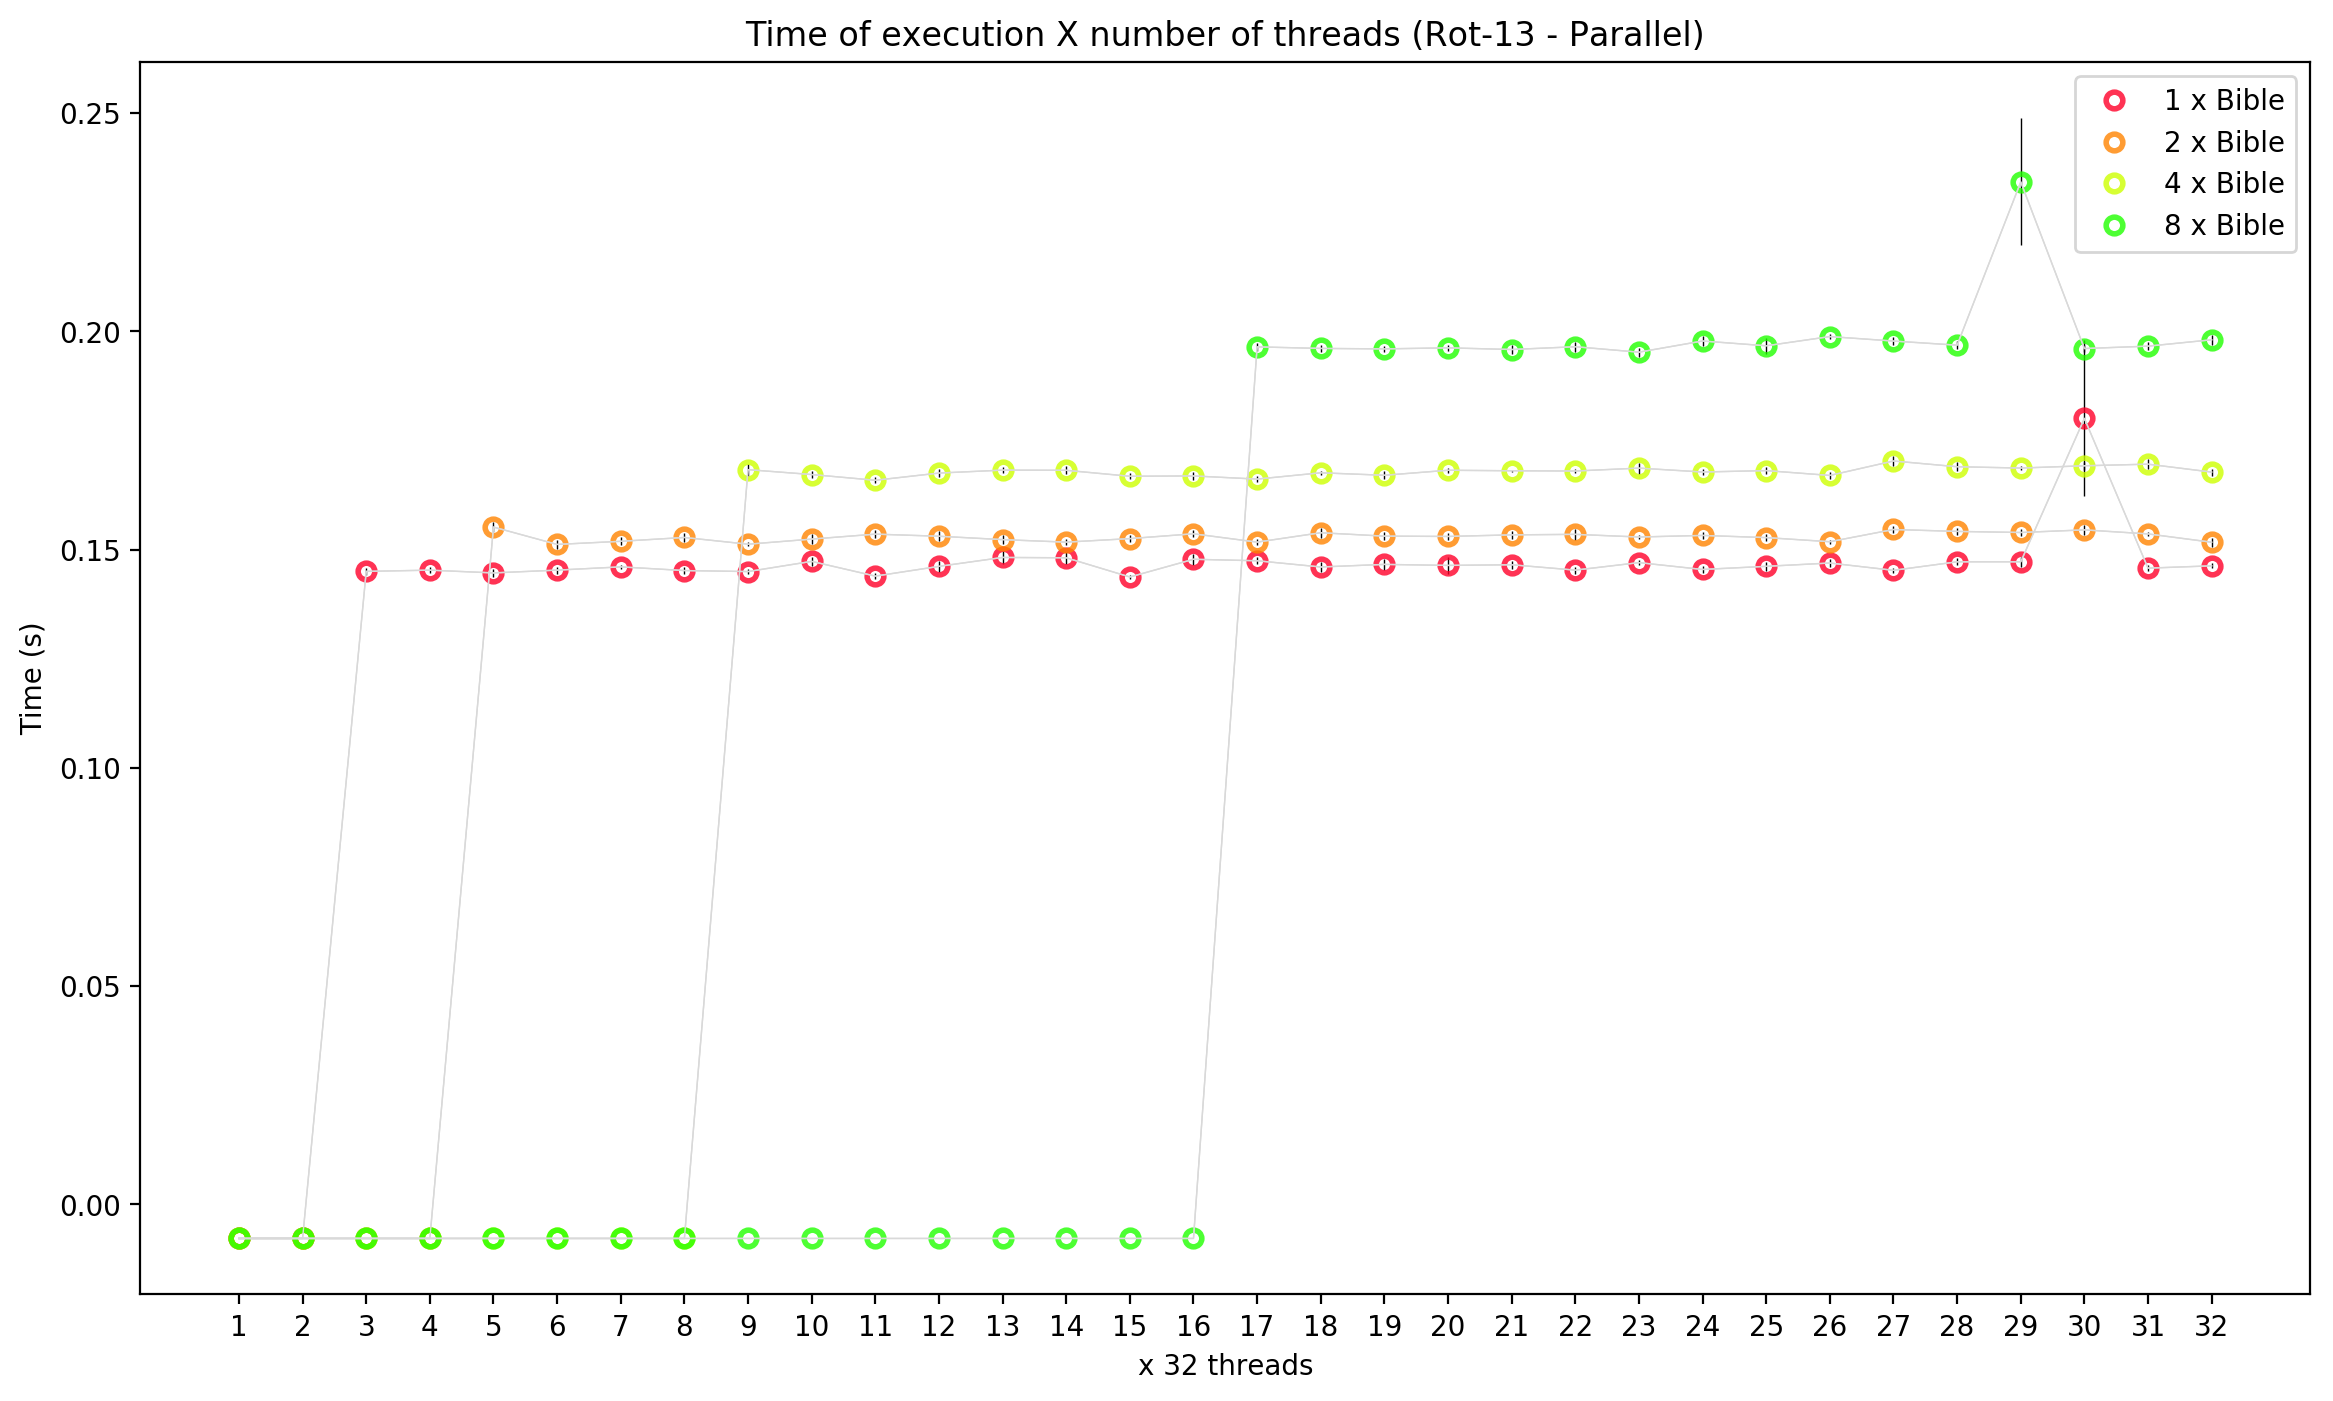
\includegraphics[scale=.55]{img/rot13_seqXpar/timeXthread_Rot-13 - Parallel.png}}
    \caption{Tempo de execução do algoritmo Rot13 paralelo variando o
    tamanho do bloco.}
\end{figure}

Nesse gráfico o eixo Y representa o tempo de execução do programa
enquanto o eixo X representa o número de threads por bloco. Para cada
tamanho de entrada uma cor é dada. Nesse gráfico fica claro como para o
mesmo tamanho de entrada, independente do número de threads por bloco o
tempo para a execução é o mesmo. No entanto o tempo cresce de acordo com
o tamanho da entrada. Esse é um resultado inesperado, pois como os 
valores são processados em paralelo não esperávamos que o tempo fosse
aumentar.

Faremos agora uma comparação entre a implementação sequencial e a paralela:

\begin{figure}[H]
    \makebox[\textwidth][c]{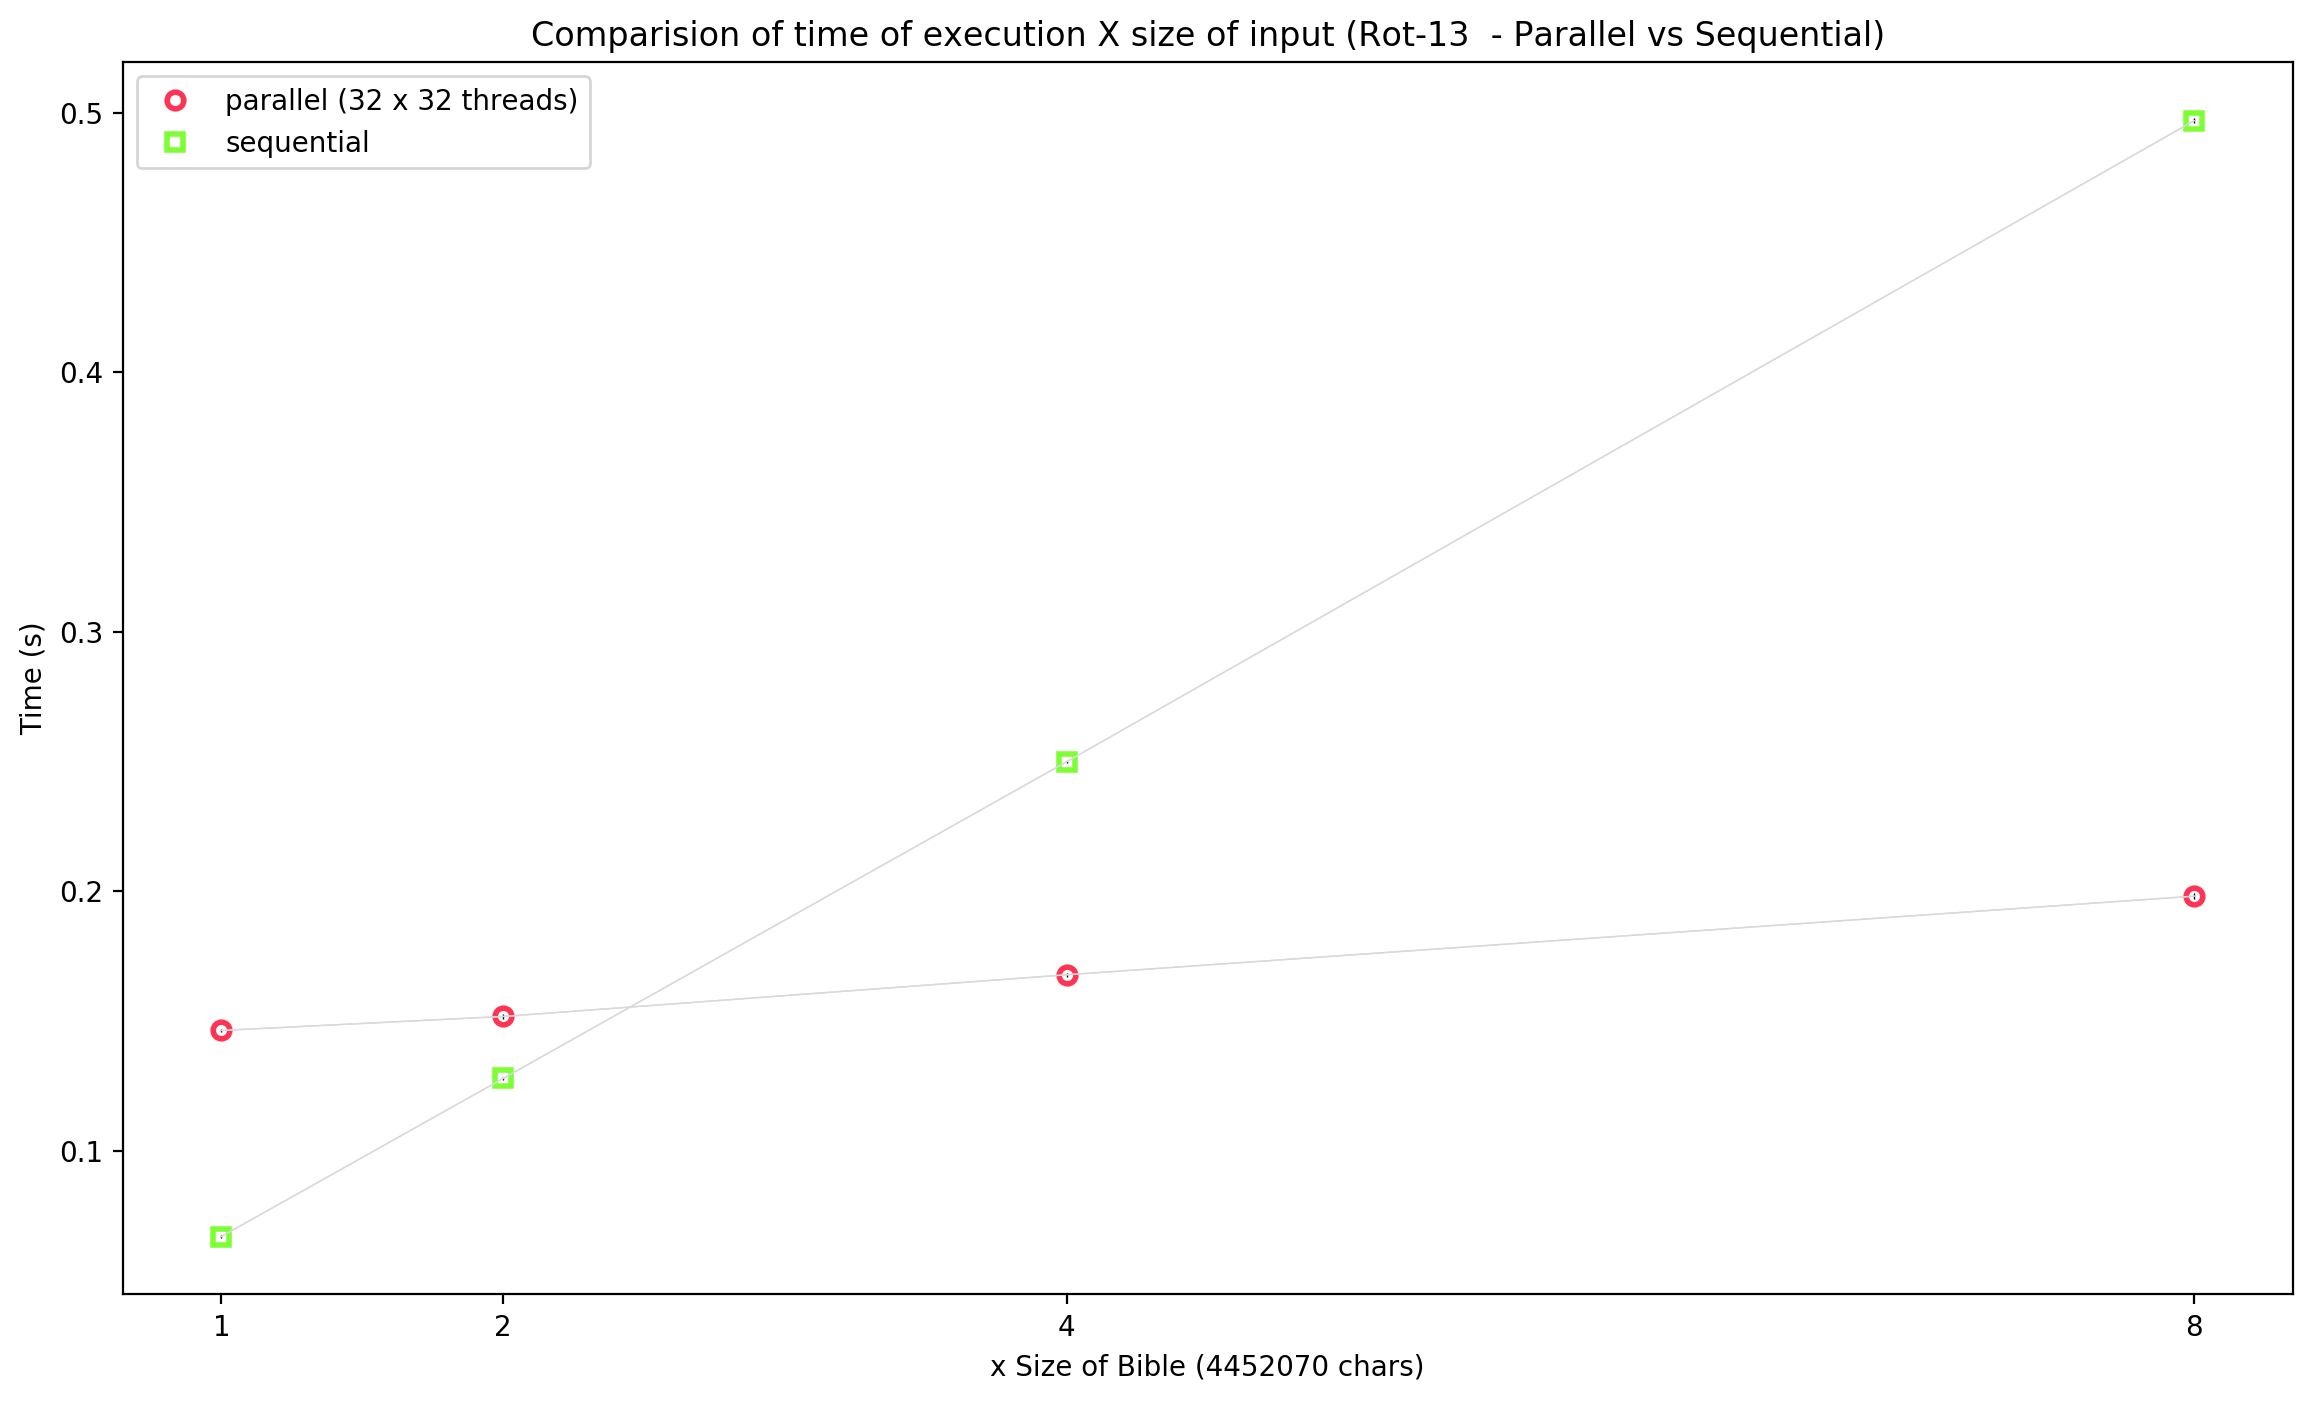
\includegraphics[scale=.55]{img/rot13_seqXpar/compare_timeXsize_Rot-13 - Parallel vs Sequential.png}}
    \caption{Comparação de tempo de execução do algoritmo Rot13 paralelo
    e sequencial.}
\end{figure}

Como discutido anteriormente, como o tempo de execução independe do
número de threads por bloco, escolhemos 32 x 32 threads, pois
garantimos que o número de blocos necessários serão validos.

Notamos um comportamento interessante, onde para 1 e 2 vezes a Bíblia,
o algoritmo sequencial é mais rápido que o paralelo. No entanto,
para valores um pouco maior que 2 vezes o tamanho da Bíblia a
implementação paralela é mais rápida. Talvez isso ocorra, devido á
transferência de dados para a GPU, que leva um tempo extra em relação à
implementação sequencial, porém como a os dados são processados
paralelamente, a taxa de crescimento do tempo em relação ao tamanho dos
arquivos de entrada da implementação paralela é menor do que o da
sequencial. De fato, talvez a implementação paralela só cresça devido a
operação de leitura de arquivo que ocorre sequencialmente para ambos os
algoritmos. Comparemos com o seguinte gráfico:

\begin{figure}[H]
    \makebox[\textwidth][c]{
        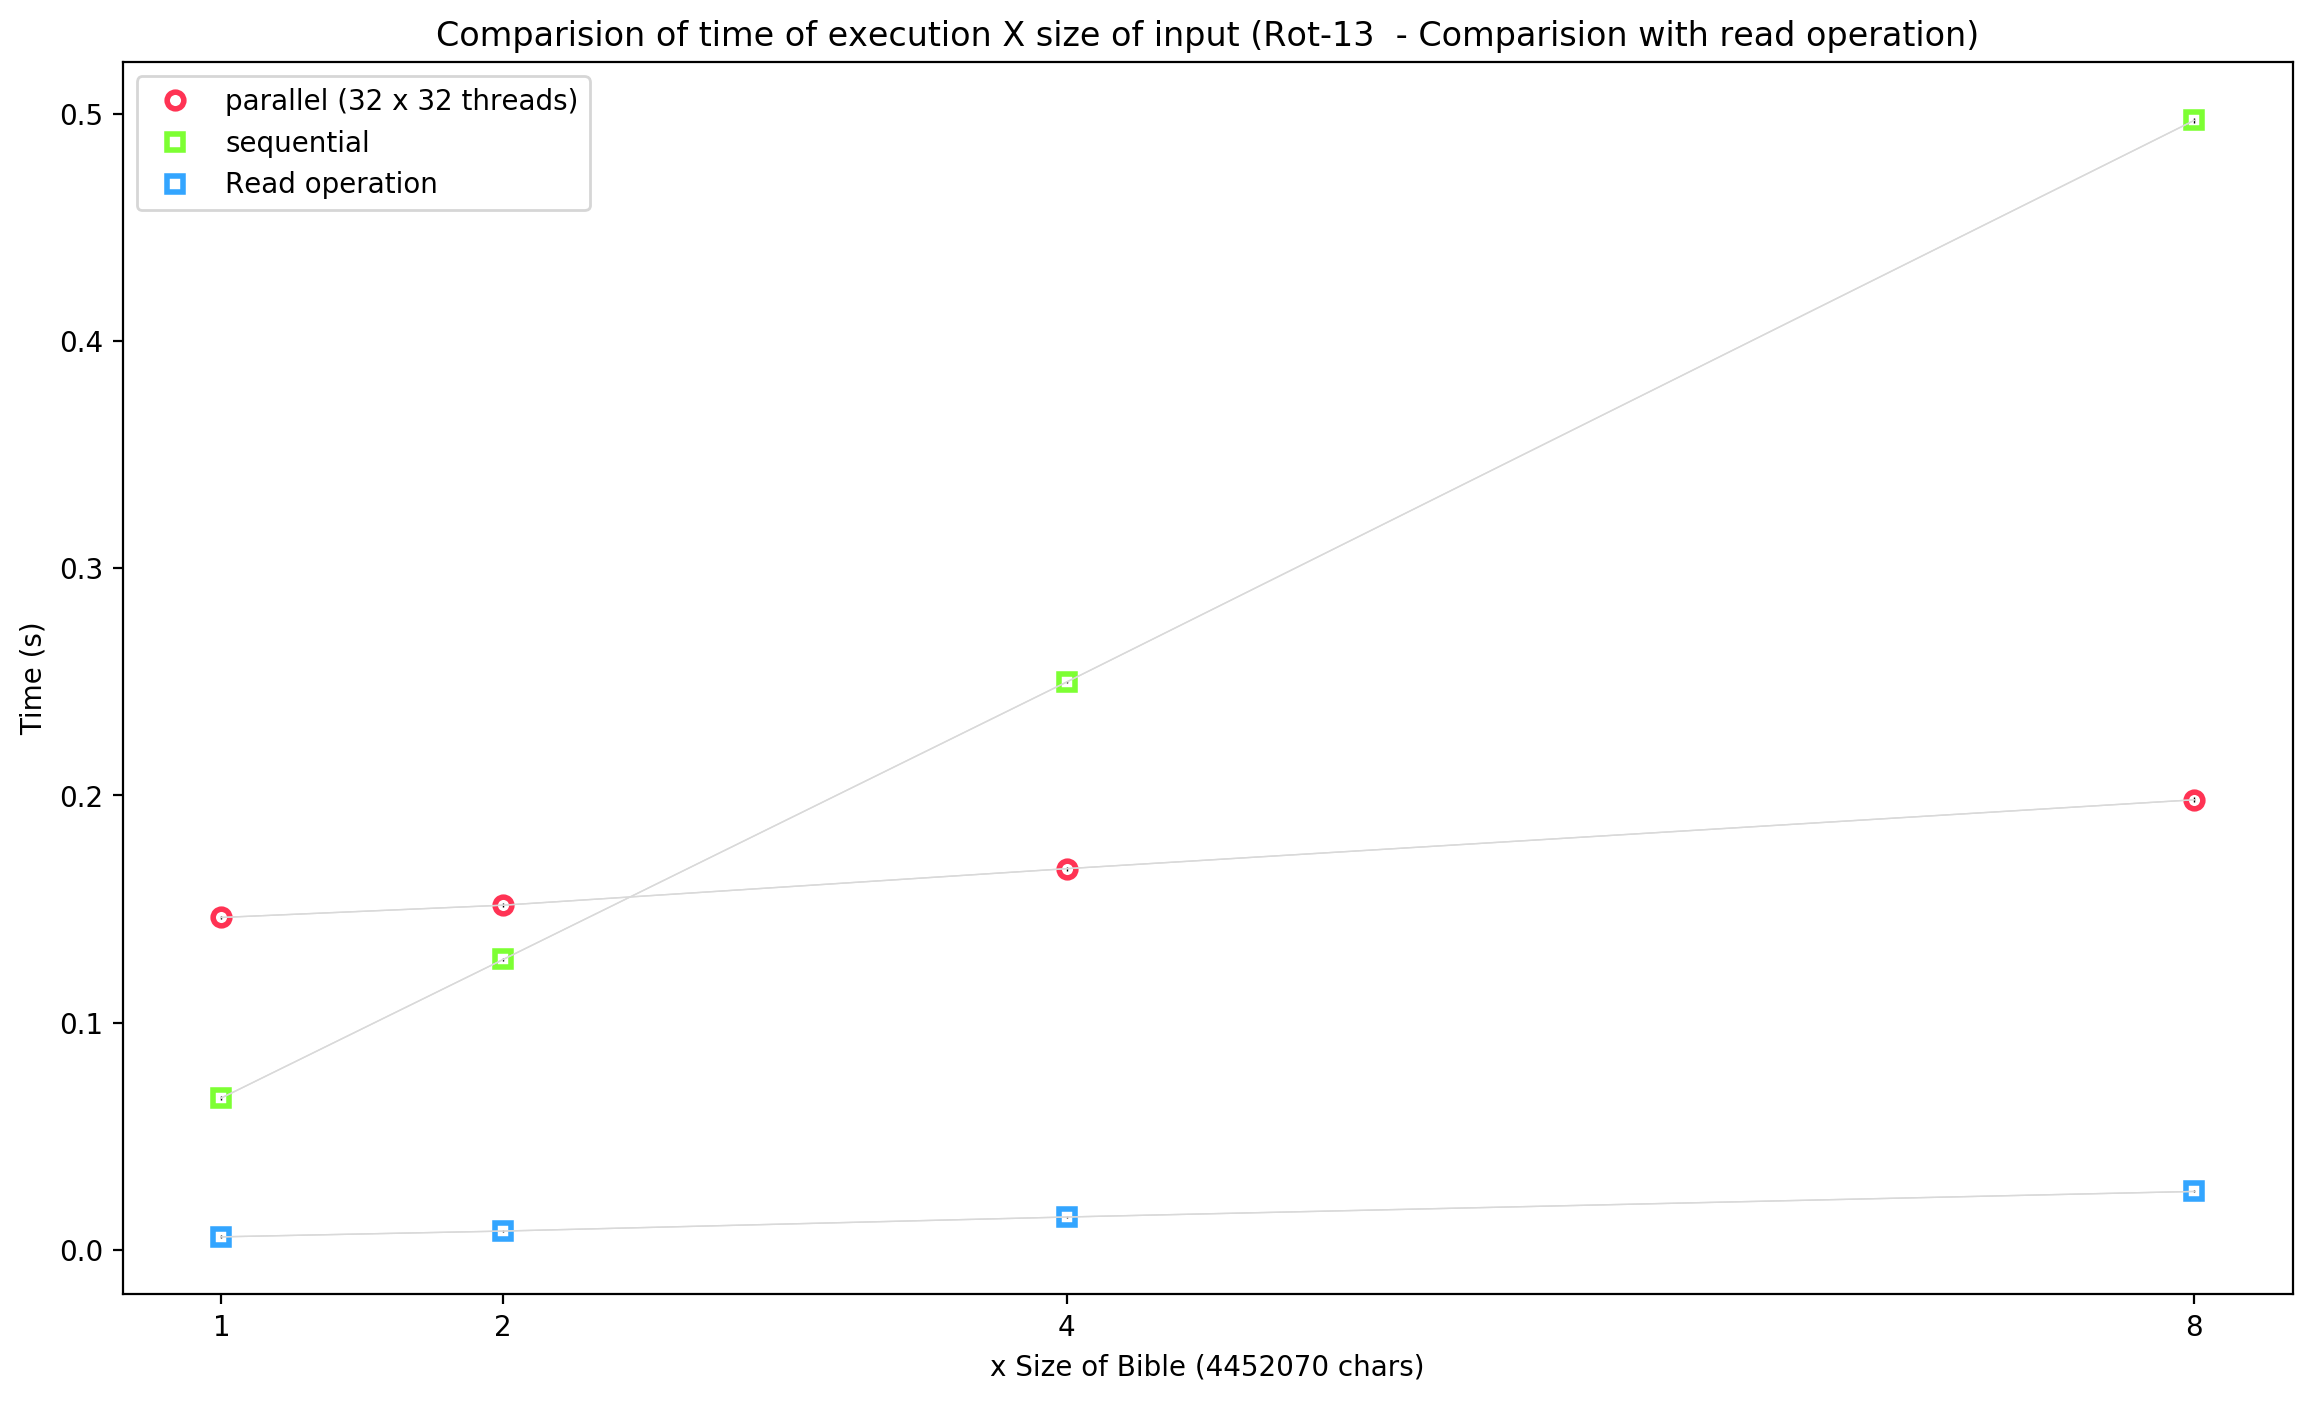
\includegraphics[scale=.55]{img/rot13_seqXpar/compare_read_Rot-13 - Comparision with read operation.png}}
    \caption{Comparação com tempo de execução com o tempo de 
        leitura da entrada.}
    \label{fig:read_operation_time}
\end{figure}

Para gerar os dados dos pontos azuis, executamos um programa que somente
lê um arquivo e o guarda em um vetor de caracteres. Essa é a mesma
função utilizada nas duas implementações do algoritmo rot13. 

Nota-se que a inclinação do tempo de leitura é bastante similar com a da
implementação paralela. Portanto se pudéssemos retirar a leitura do 
algoritmo paralelo, o tempo para encriptação seria o mesmo independente
do tamanho de entrada. É claro que isso se limita aos valores máximos
de threads por bloco e de blocos por GPU. 

\subsection{Vigenere}
A primeira observação que fizemos é que o algoritmo sequencial tem 
complexidade linear com o tamanho da entrada, como podemos ver na 
figura \ref{fig:vigenere_seqtime}. Esse desempenho já era 
esperado dado que ler o texto é feito linearmente assim como a 
encriptação em si.

\begin{center}
\begin{figure}[H]
    \makebox[\textwidth][c]{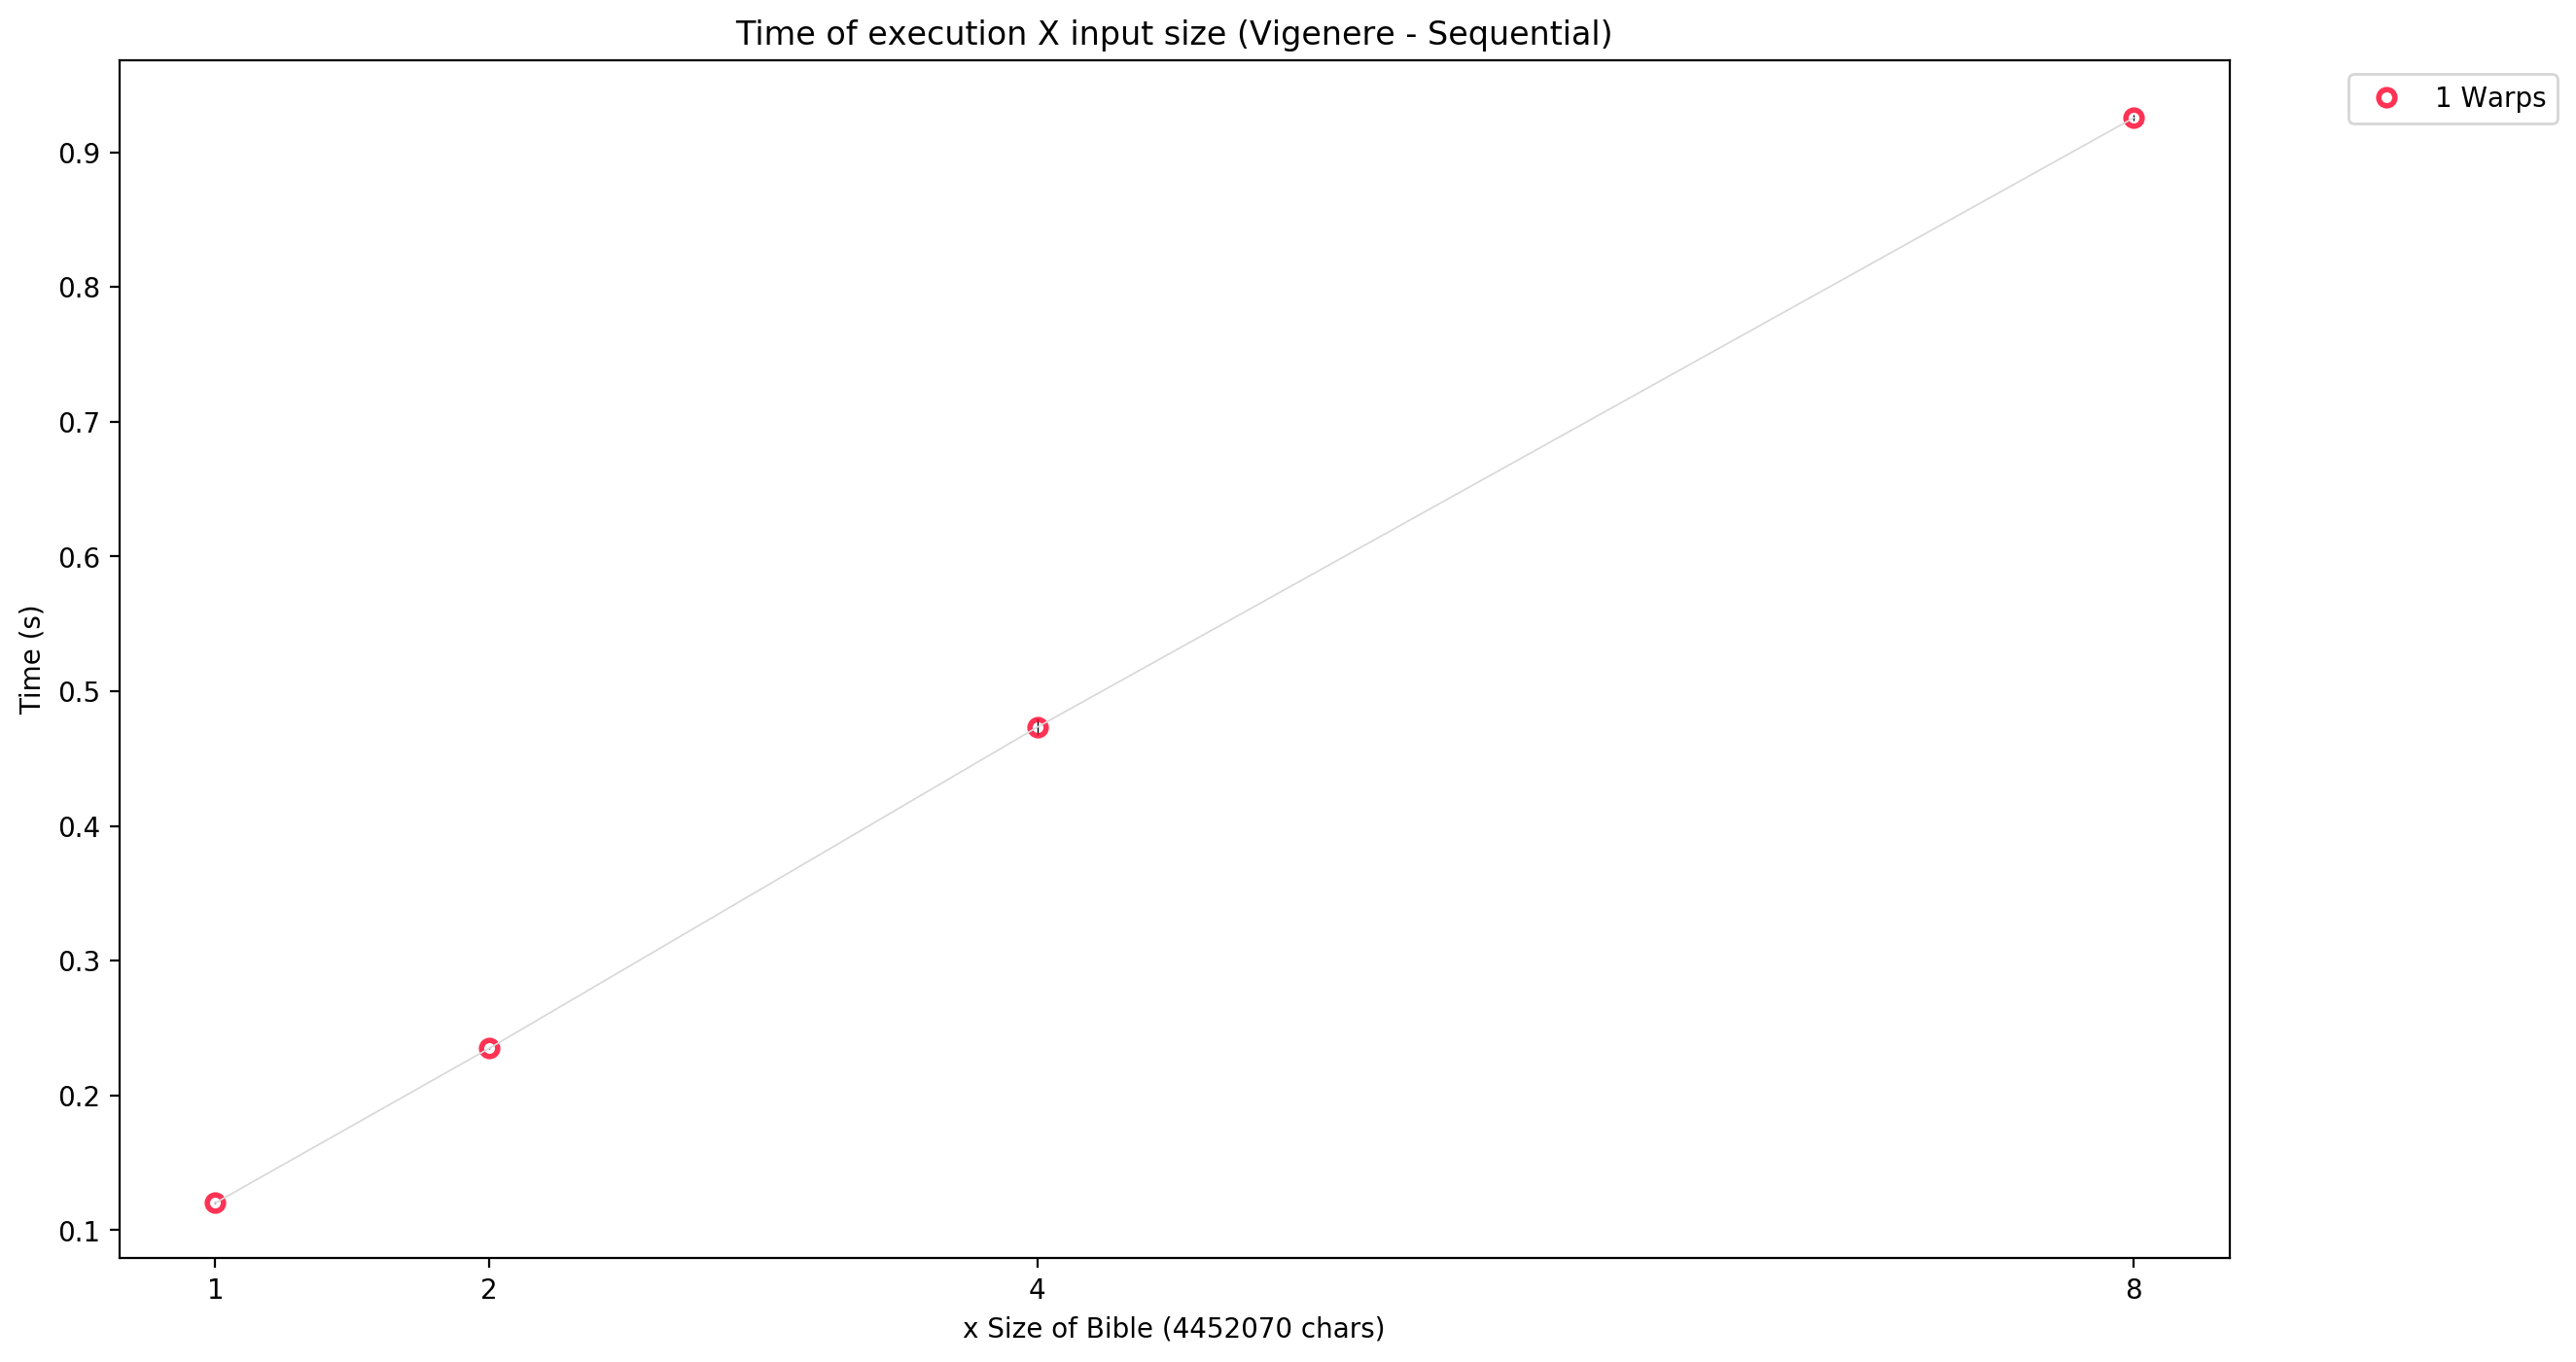
\includegraphics[scale=.45]{img/vigenere/time_seq.png}}
    \caption{Tempo de execução do algoritmo Vigenere sequencial.}
    \label{fig:vigenere_seqtime} 
\end{figure}
\end{center}

Assim como no algoritmo Rot13, percebemos que o tempo de execução não 
aumenta muito conforme aumentamos o tamanho da entrada. Inclusive, como
observamos na imagem \ref{fig:read_operation_time}, essa inclinação se 
deve, em boa parte, pela operação de leitura de texto em arquivo.

\begin{figure}[H]
    \makebox[\textwidth][c]{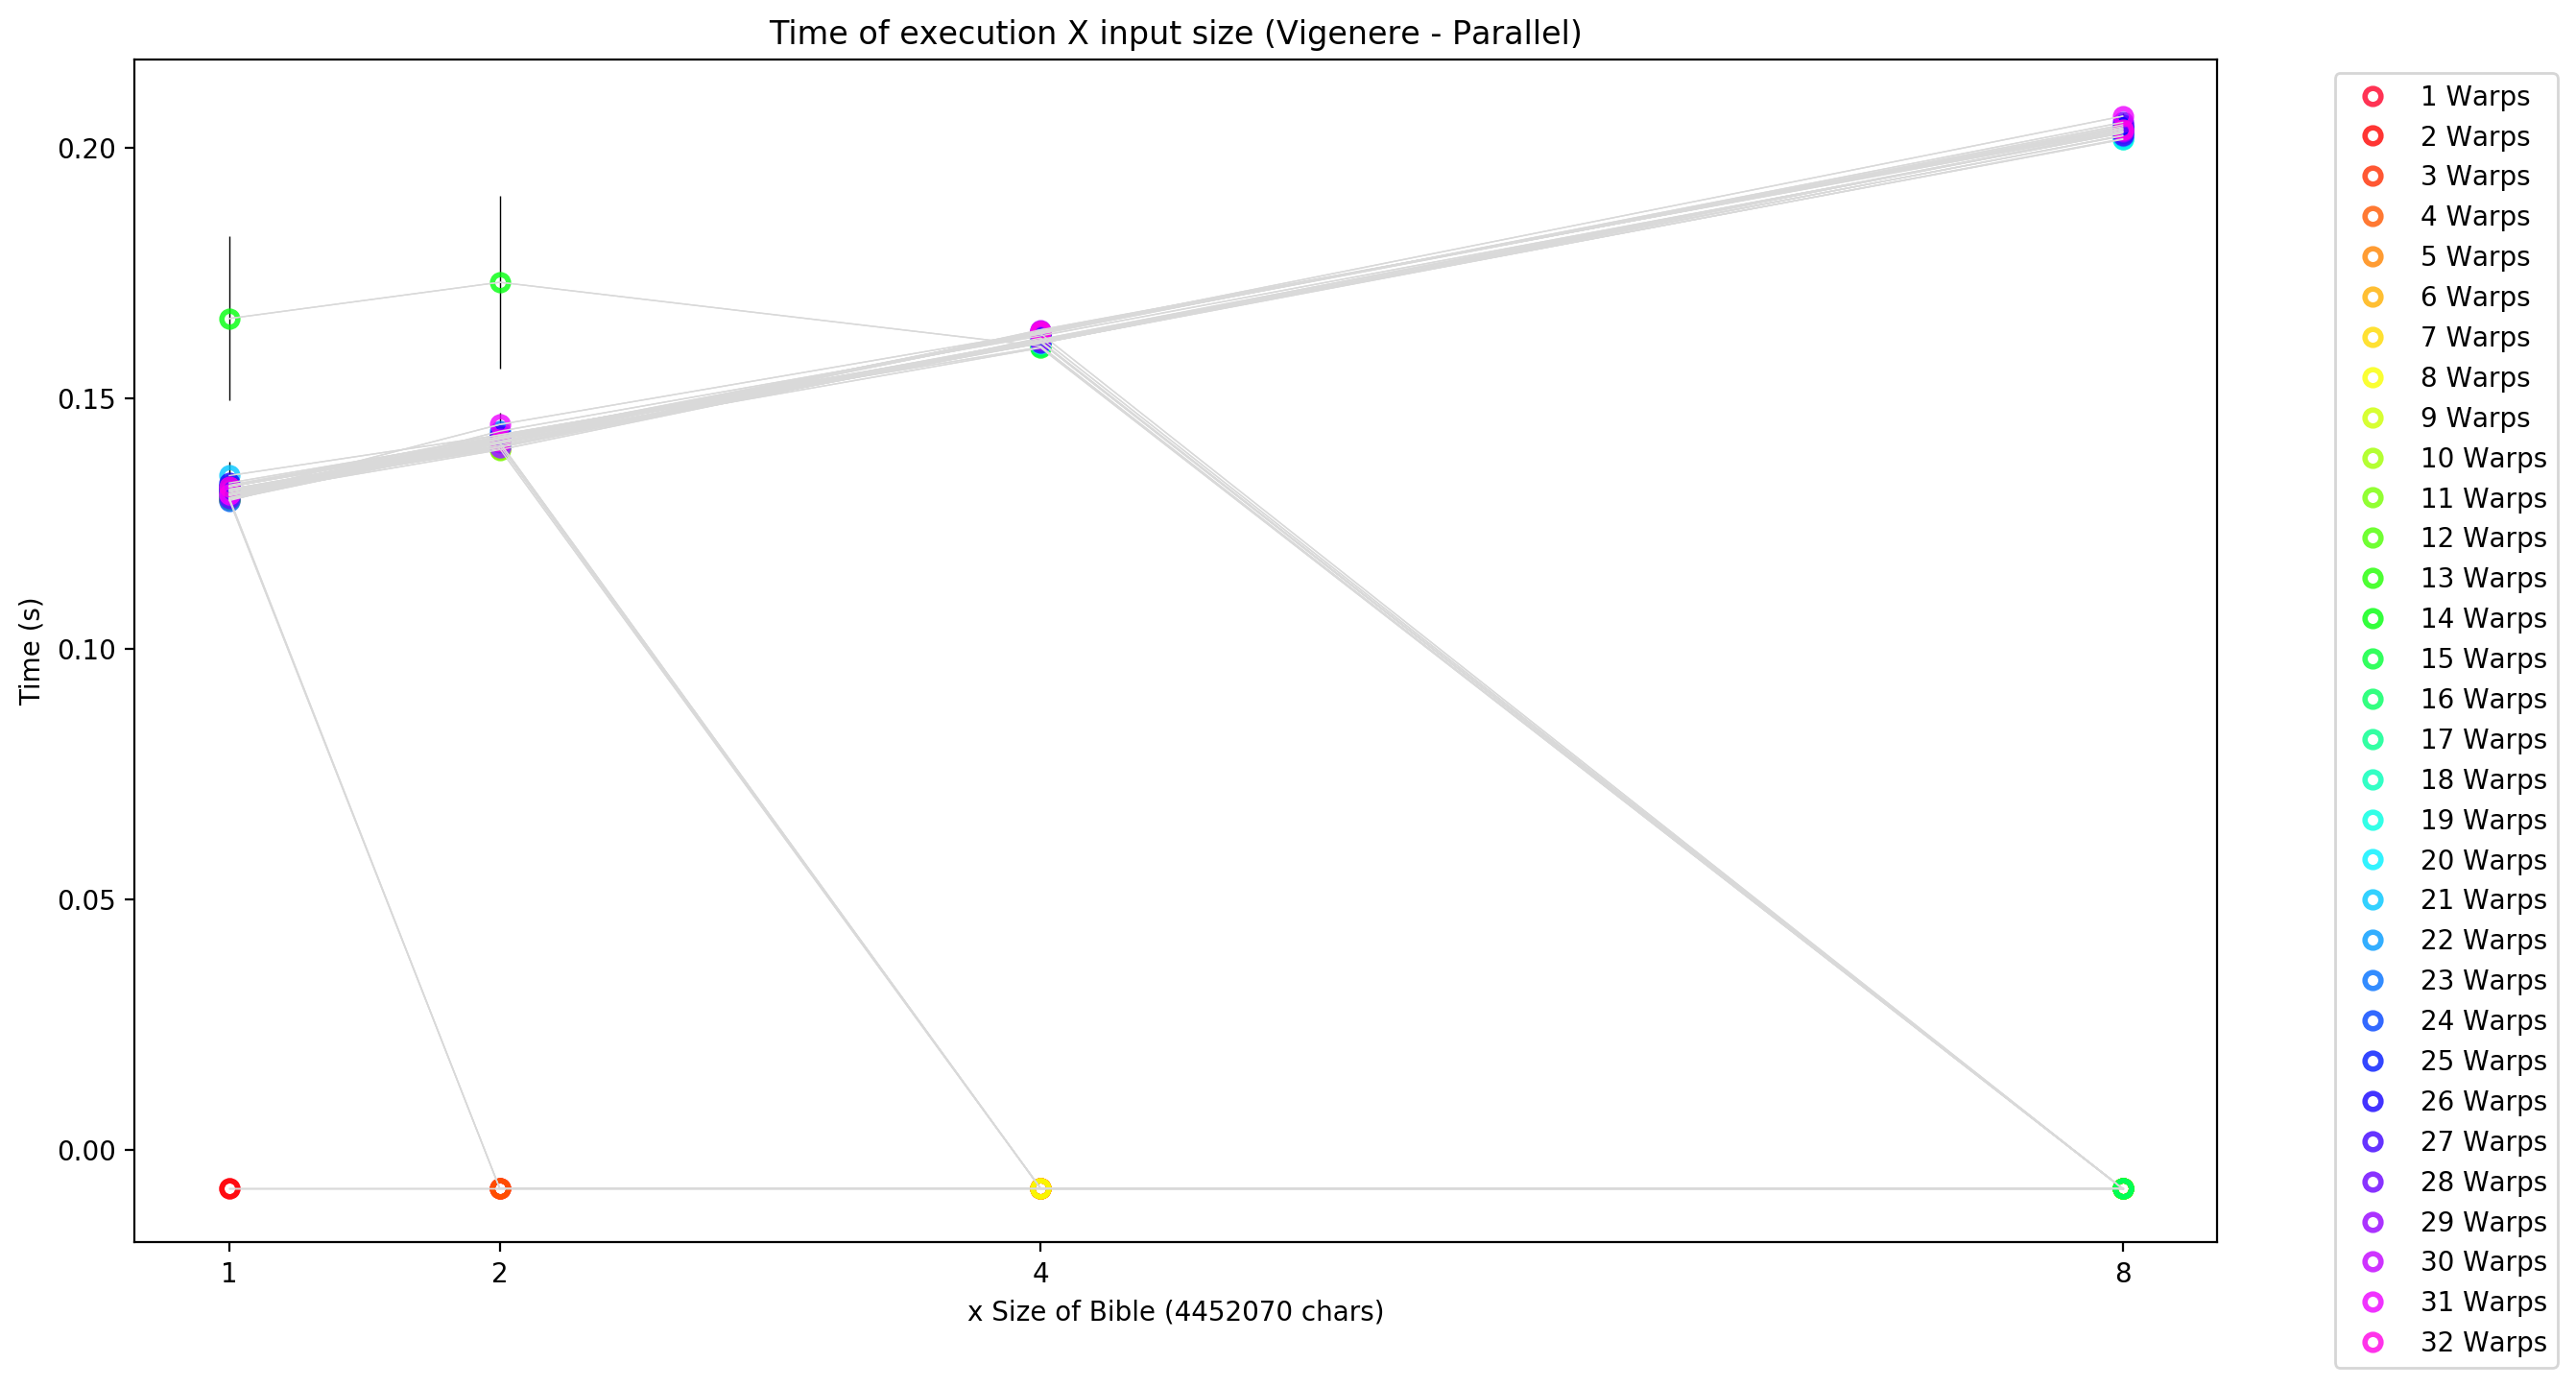
\includegraphics[scale=.45]{img/vigenere/timexsize.png}}
    \caption{Tempo de execução do algoritmo Vigenere paralelo variando o
    tamanho de entrada. Note que os pontos que marcam abaixo de zero 
    segundos se referem a instâncias do problema que não rodaram na GPU
    por excederem limites como número máximo de blocos.}
\end{figure}

Novamente como no caso Rot13, quando aumentamos o número de threads por
bloco o desempenho continua muito parecido.

\begin{figure}[H]
    \makebox[\textwidth][c]{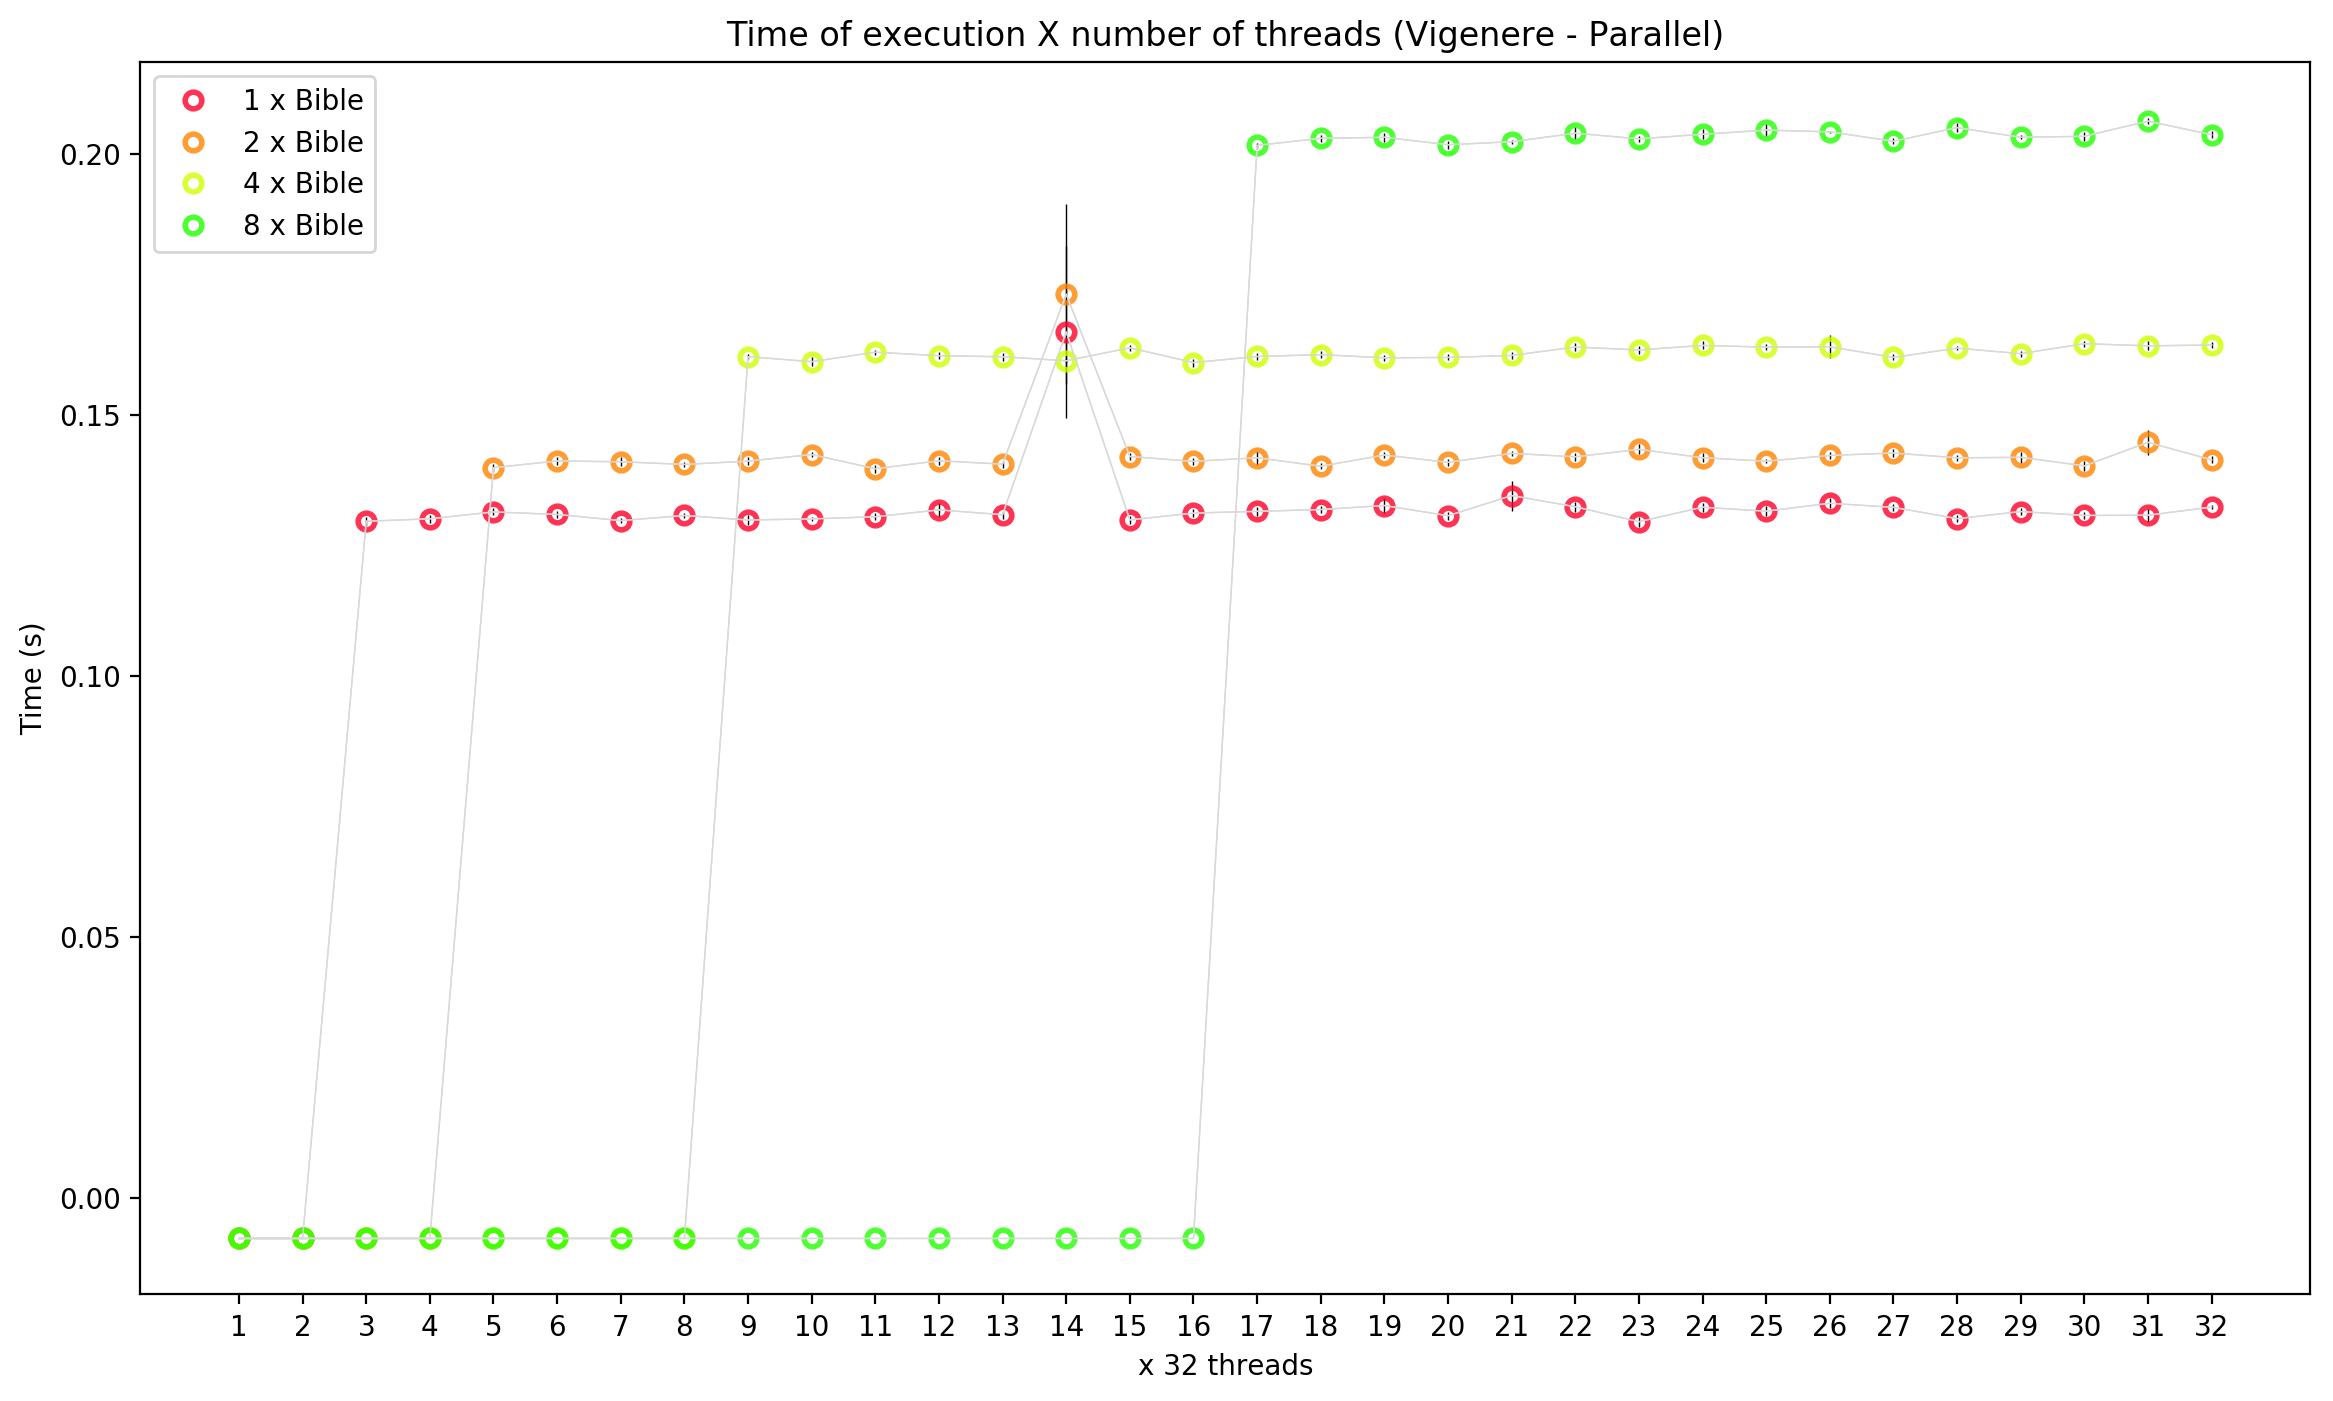
\includegraphics[scale=.45]{img/vigenere/timexthread.png}}
    \caption{Tempo de execução do algoritmo Vigenere paralelo variando o
    tamanho do bloco. Note que os pontos que marcam abaixo de zero se
    referem a instâncias do problema que não rodaram na GPU porque 
    excedem limites como o número máximo de blocos.}
\end{figure}


Quando comparamos as versões paralelas e sequenciais do programa, 
percebemos que para as entradas maiores o algoritmo paralelo é melhor do
que o algoritmo sequencial. Isto é, quando aumentamos a quantidade de 
computação necessária, o overhead da estrutura de paralelismo é pago
pelos ganhos em velocidade dos cálculos.


\begin{figure}[H]
    \makebox[\textwidth][c]{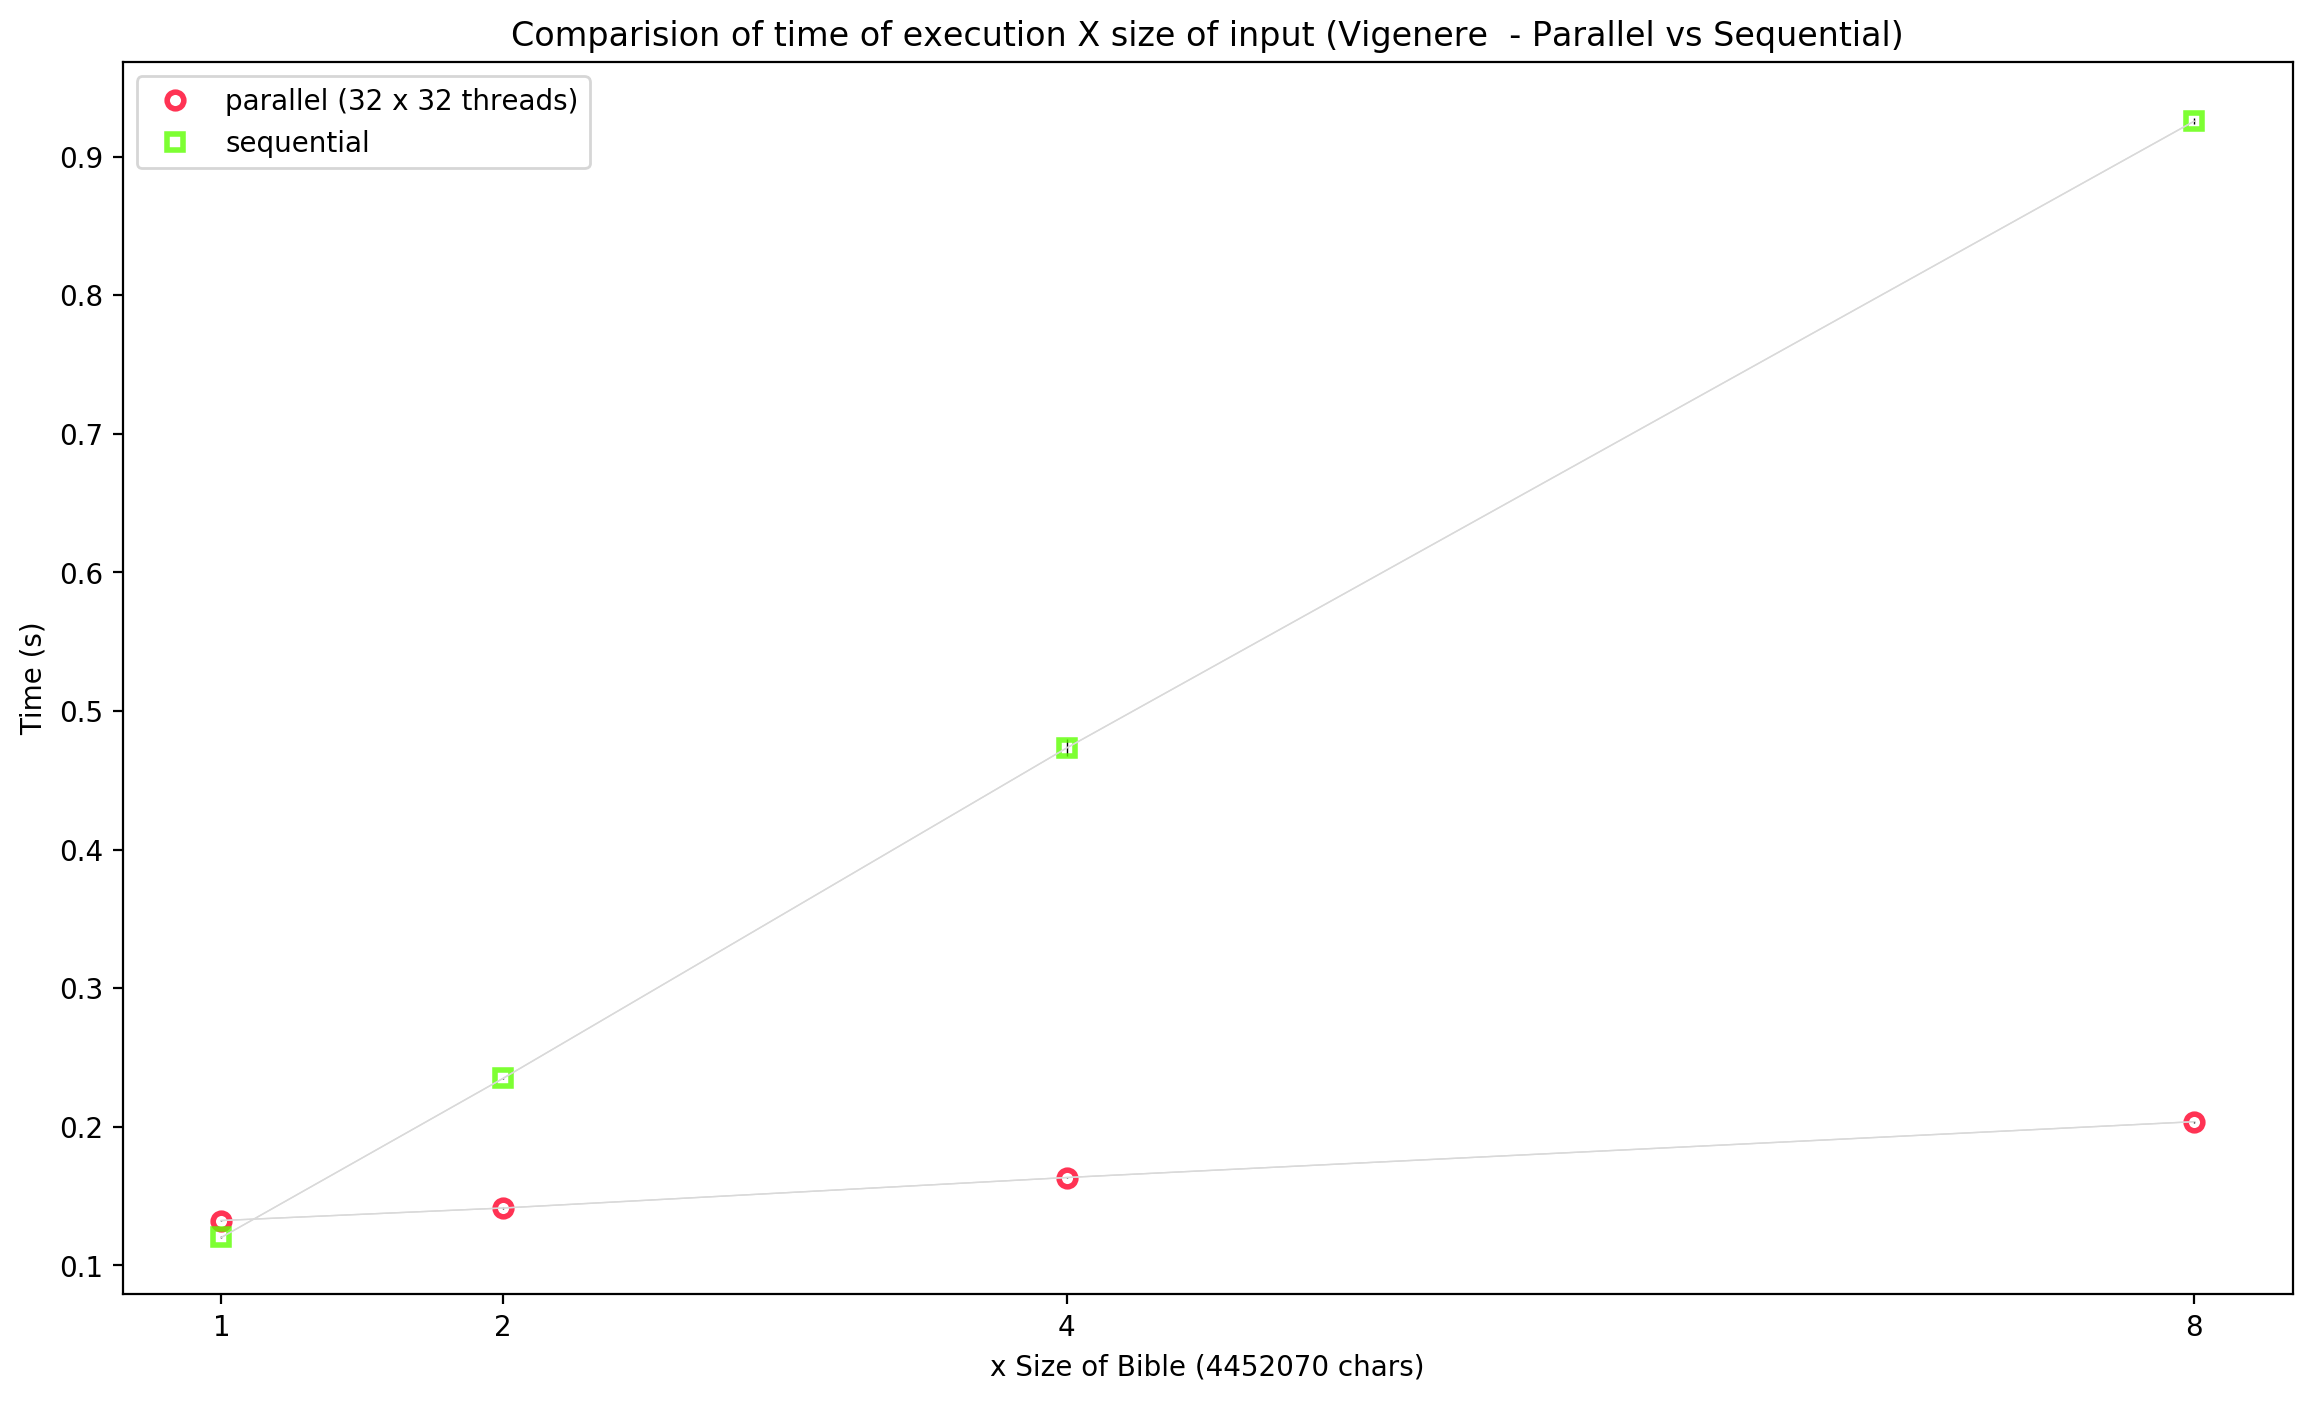
\includegraphics[scale=.45]{img/vigenere/parallelxseq.png}}
    \caption{Comparação de tempo de execução do algoritmo Vigenere
    paralelo e sequencial.}
\end{figure}


\subsection{Base64}
A implementação sequencial do algoritmo Base64 mostrou, como esperado
um comportamento linear conforme o tamanho da entrada.

\begin{center}
\begin{figure}[H]
    \makebox[\textwidth][c]{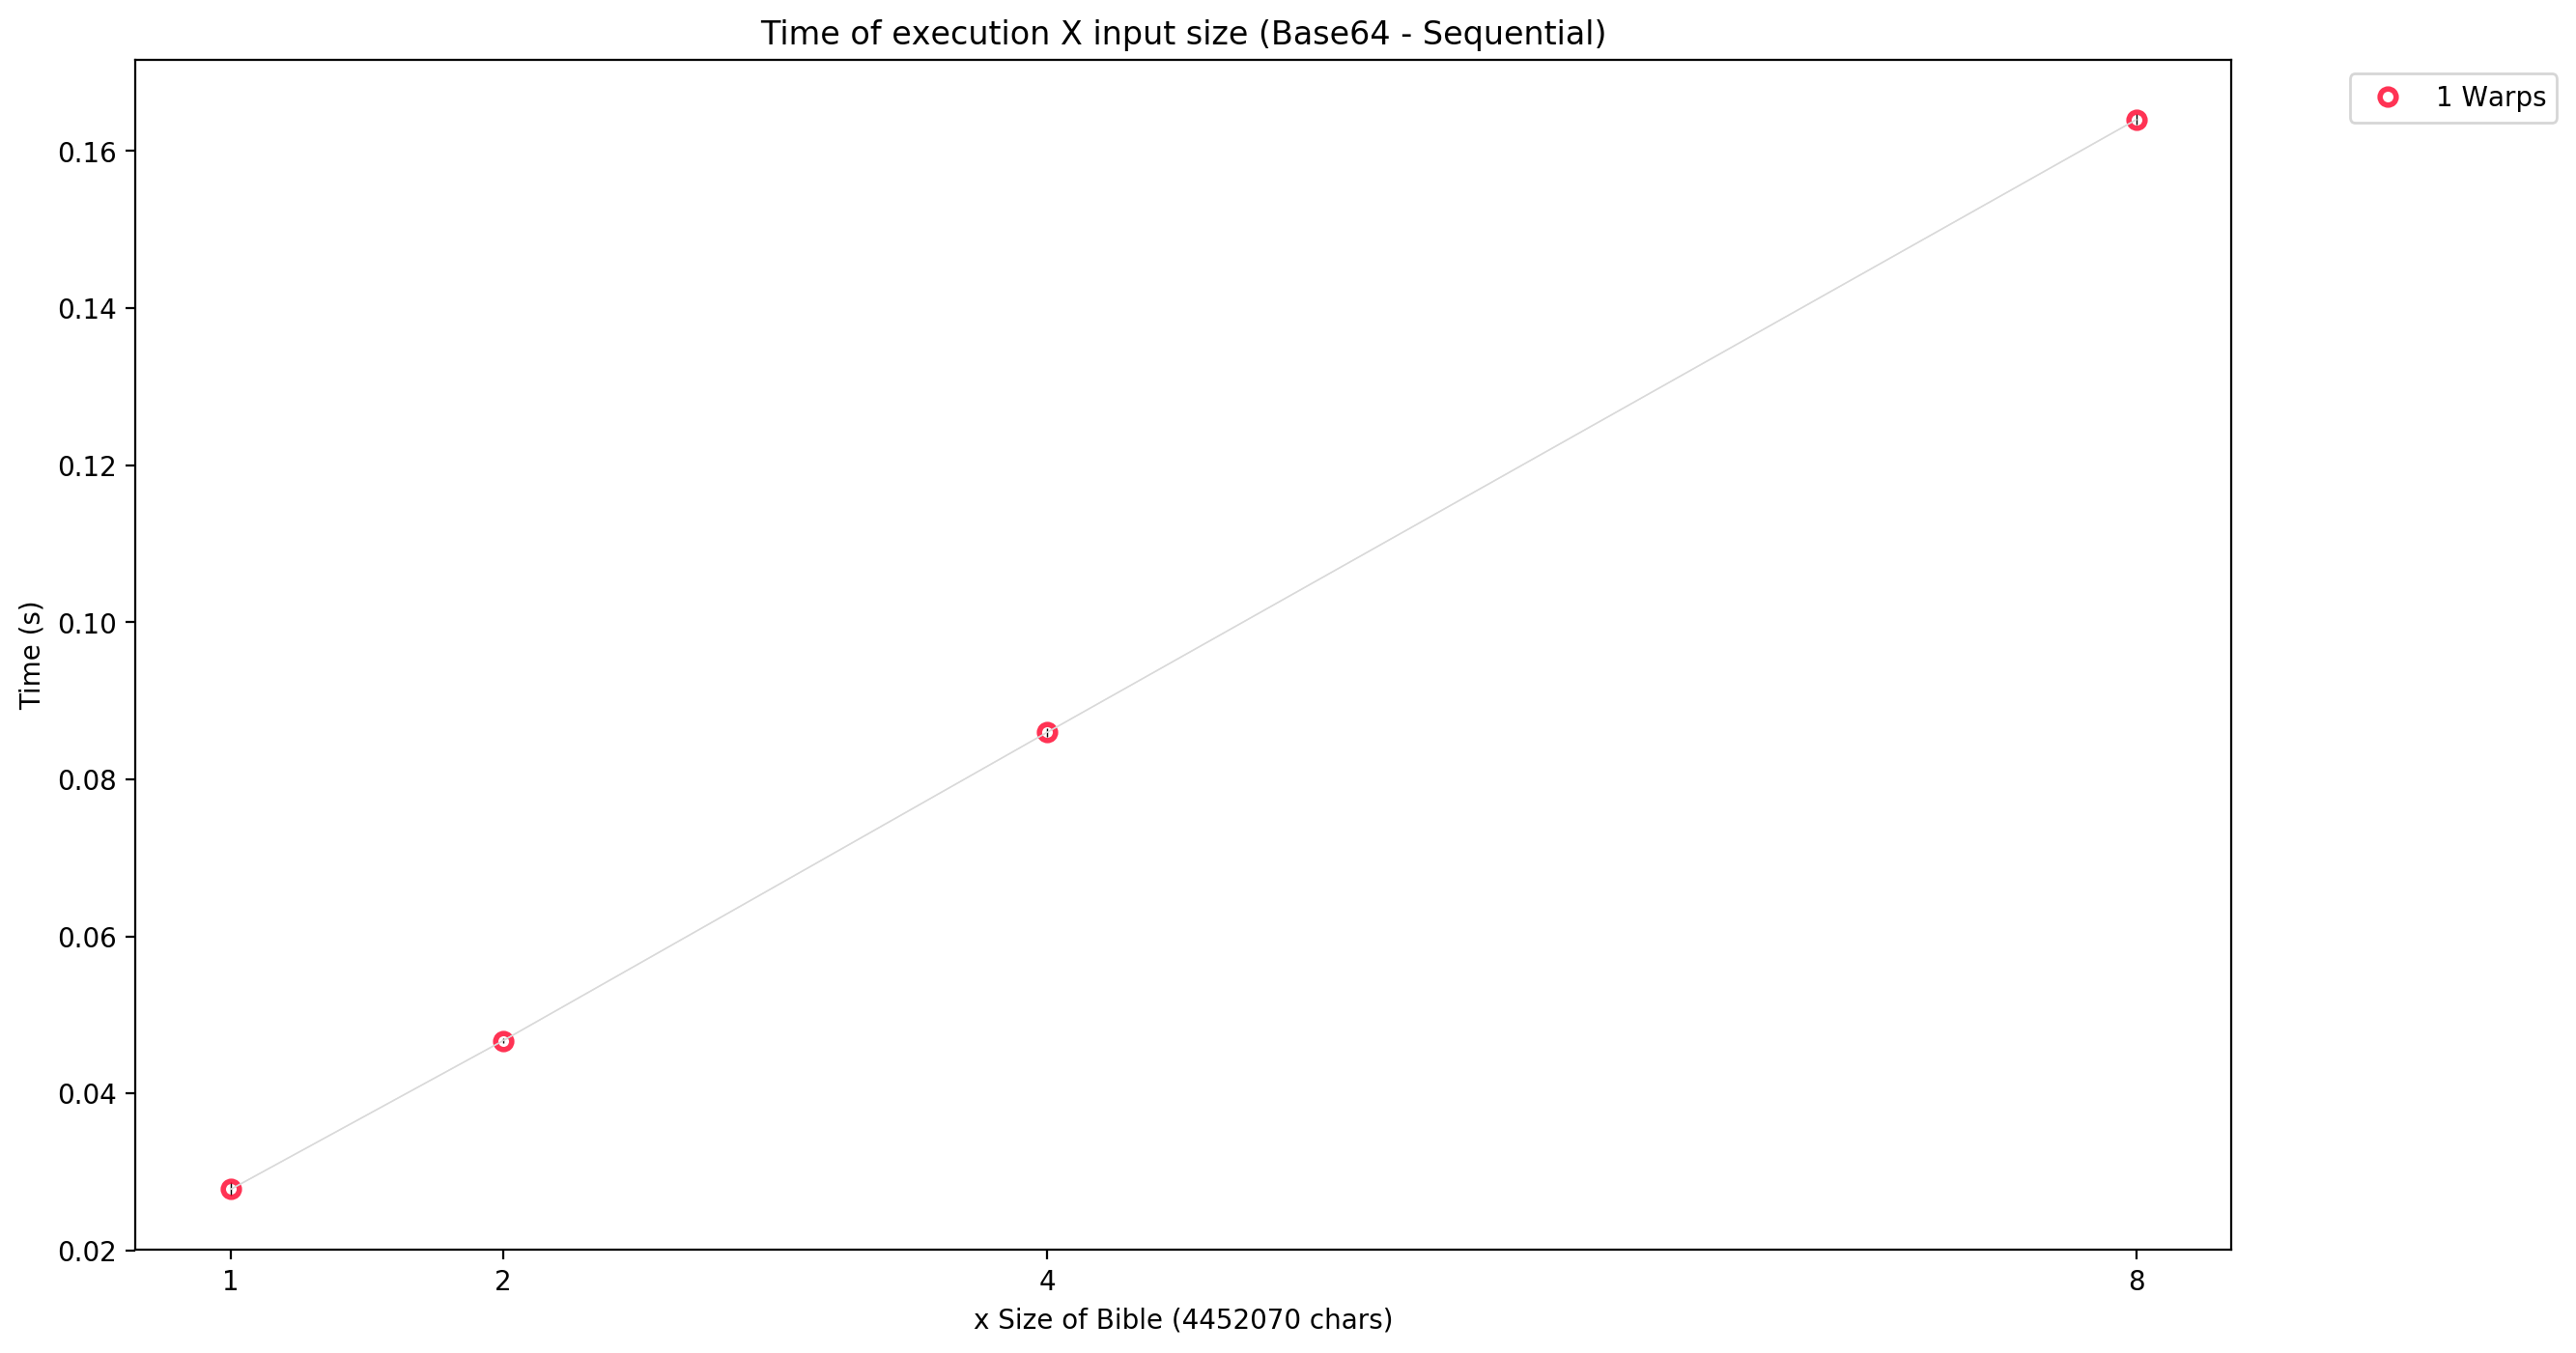
\includegraphics[scale=.45]{img/base64/time_seq.png}}
    \caption{Tempo de execução do algoritmo Base64 sequencial.}
    \label{fig:vigenere_seqtime} 
    %todo: fix this image
\end{figure}
\end{center}

Assim como no algoritmo Rot13 e Vigenere, percebemos que o tempo
de execução não aumenta muito conforme aumentamos o tamanho da entrada. 
Inclusive, como observamos na imagem \ref{fig:read_operation_time}, 
essa inclinação se deve, em boa parte, pela operação de leitura de texto
em arquivo.

\begin{figure}[H]
    \makebox[\textwidth][c]{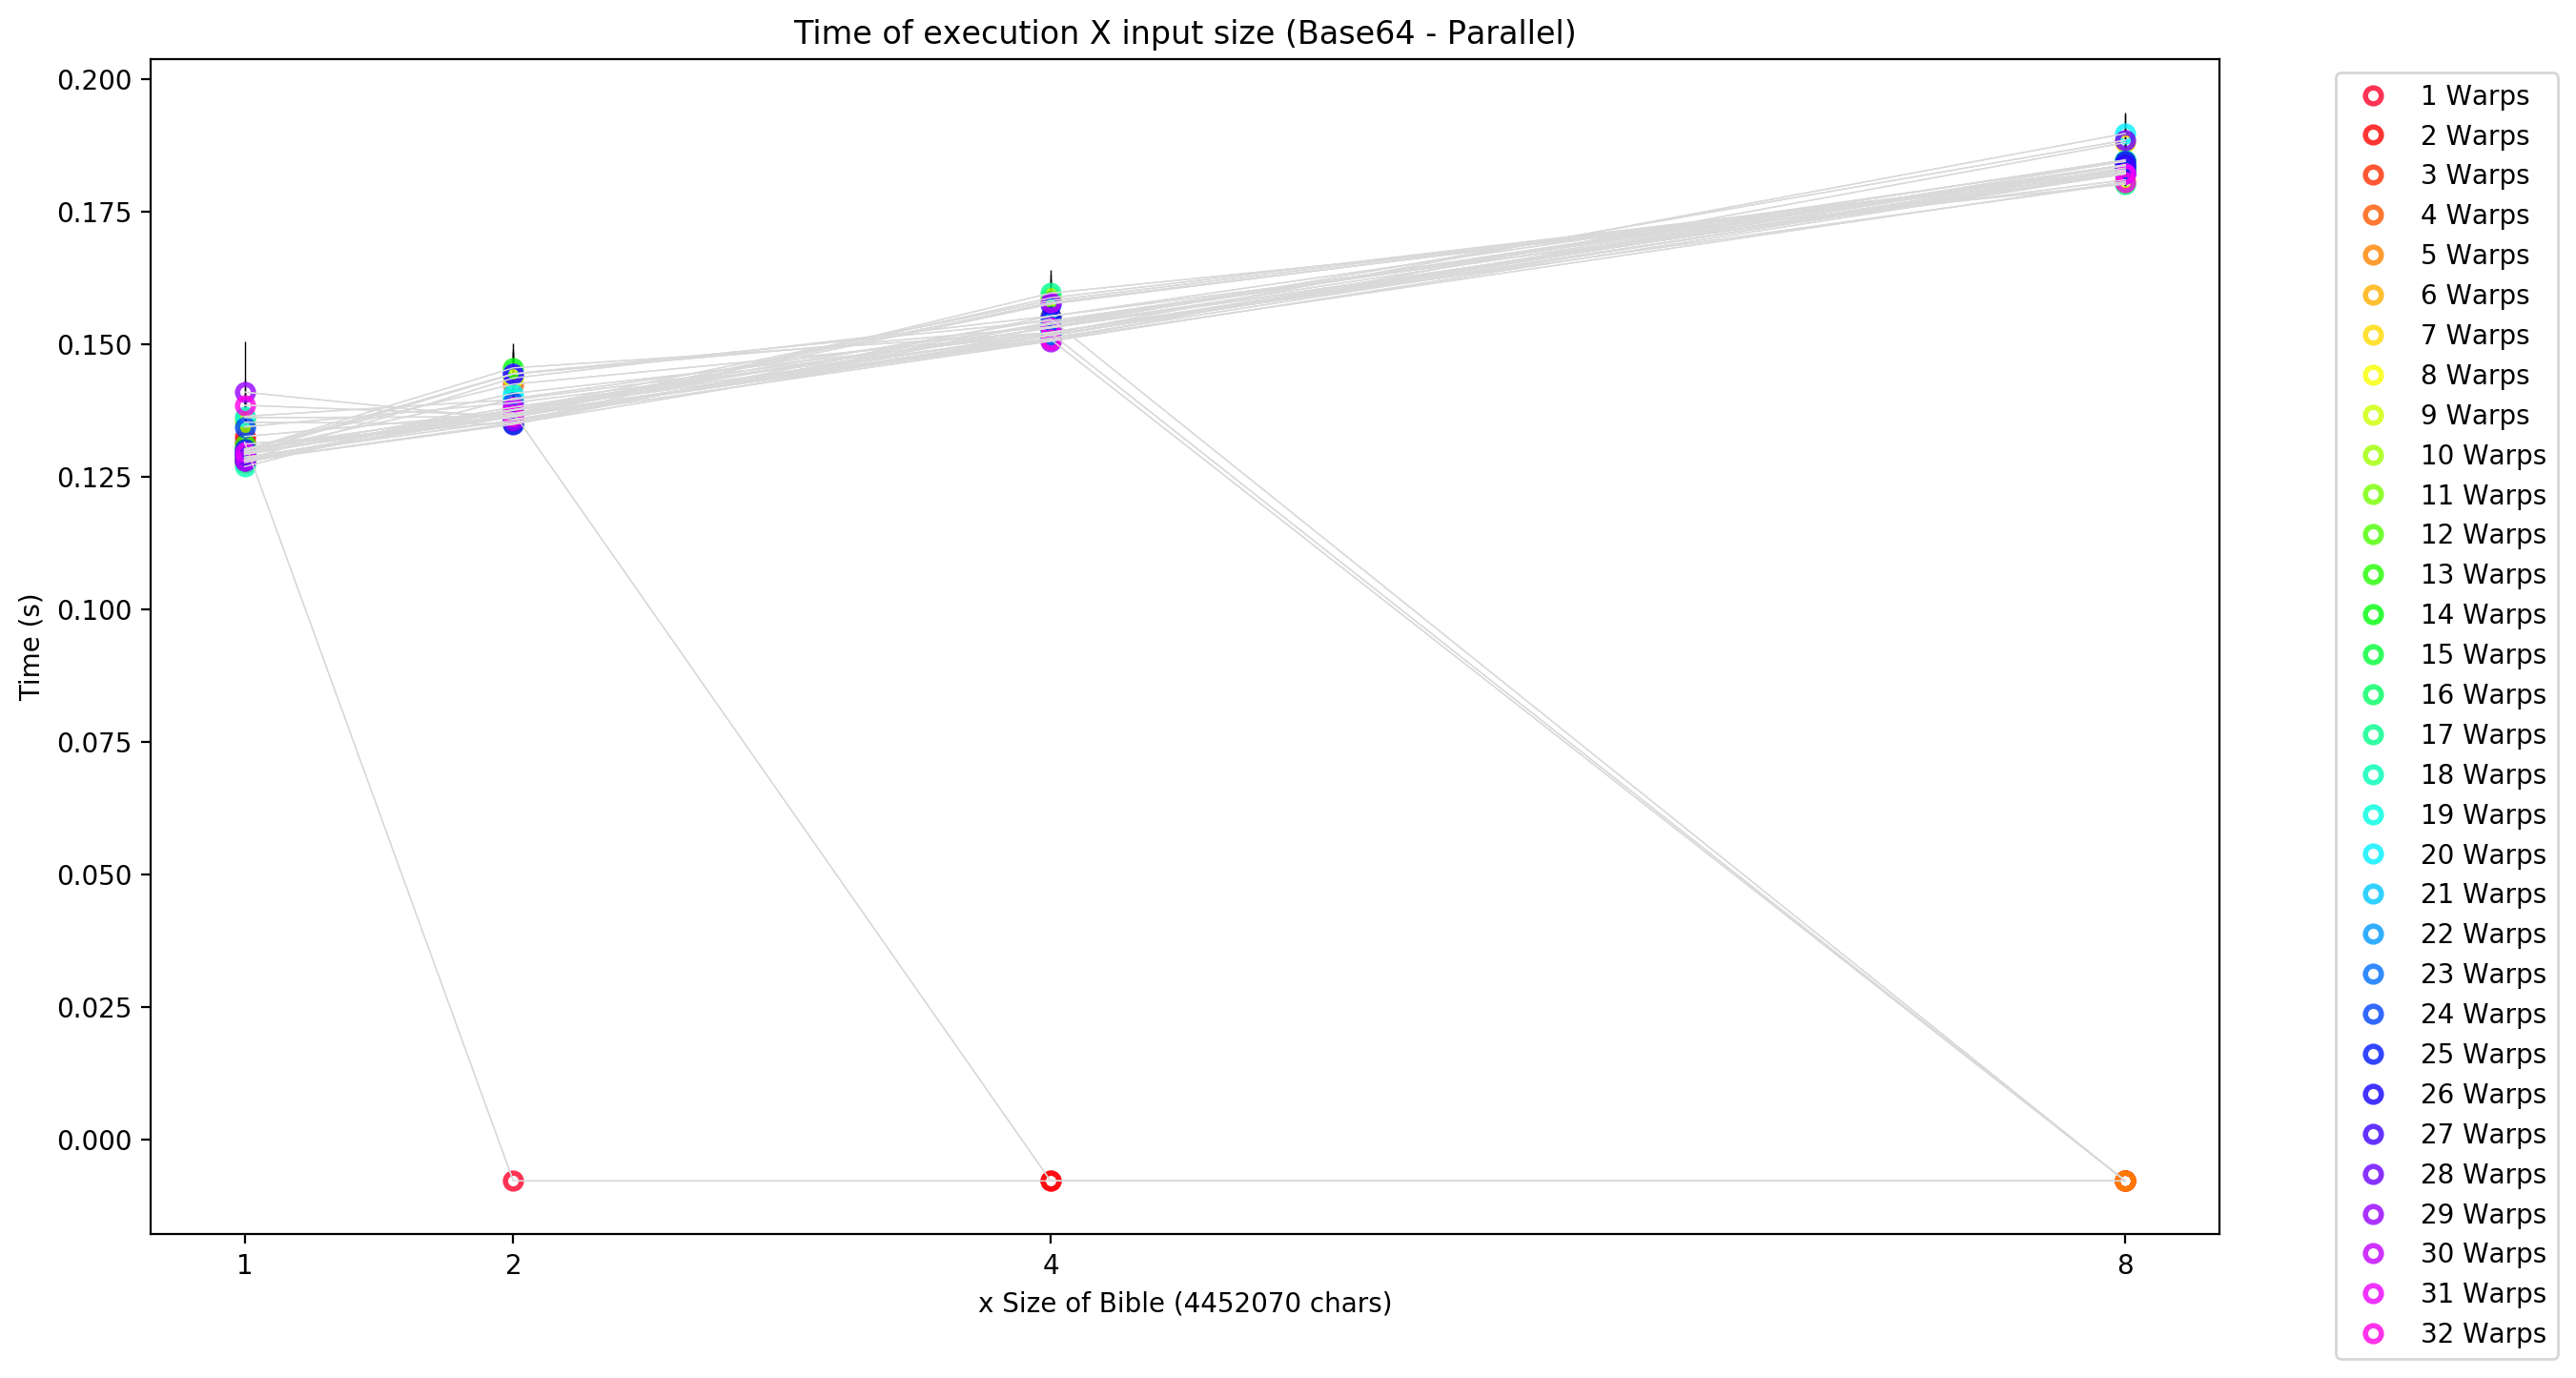
\includegraphics[scale=.45]{img/base64/timexsize.png}}
    \caption{Tempo de execução do algoritmo Base64 paralelo variando o
    tamanho de entrada. Note que os pontos que marcam abaixo de zero 
    segundos se referem a instâncias do problema que não rodaram na GPU
    por excederem limites como número máximo de blocos.}
\end{figure}

Novamente, assim como nos algoritmos Rot13 e Vigenere, quando aumentamos
o número de threads por bloco o desempenho continua muito parecido.

\begin{figure}[H]
    \makebox[\textwidth][c]{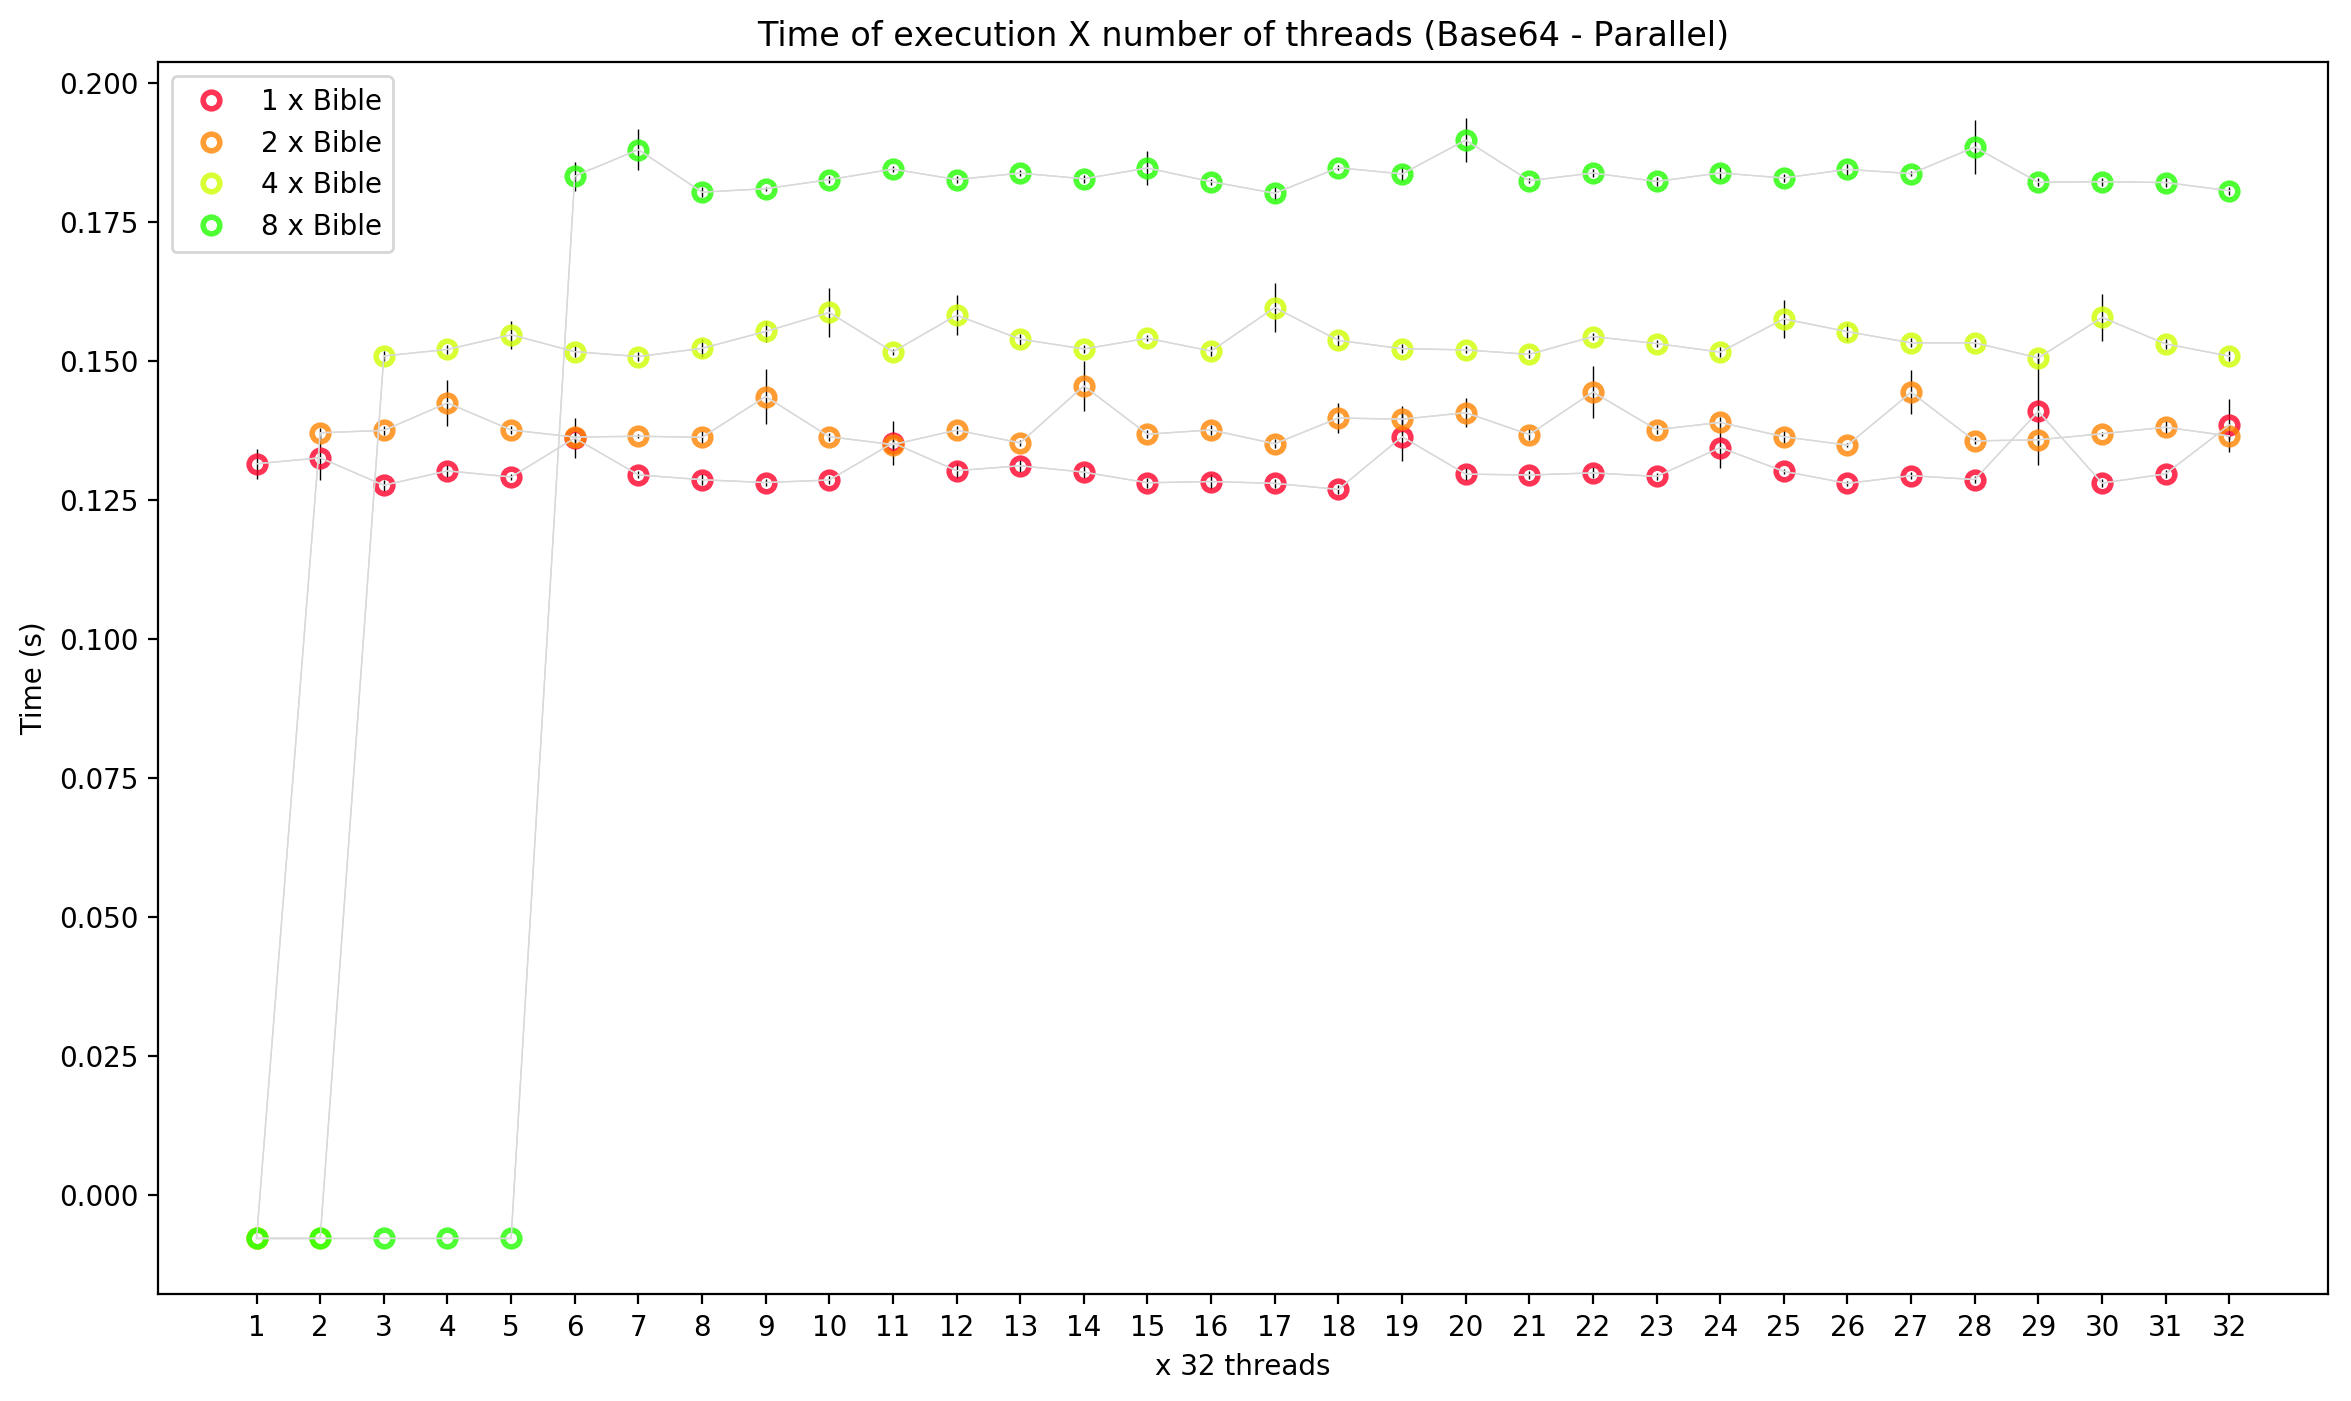
\includegraphics[scale=.45]{img/base64/timexthread.png}}
    \caption{Tempo de execução do algoritmo Base64 paralelo variando o
    tamanho do bloco. Note que os pontos que marcam abaixo de zero se
    referem a instâncias do problema que não rodaram na GPU porque 
    excedem limites como o número máximo de blocos.}
\end{figure}

Porém, quando comparamos o Base64 paralelo com o sequêncial, observamos
que a implementação sequencial teve desempenho melhor do que a versão
paralela, diferente dos outros algoritmos. Concluimos que isso aconteceu
simplismente porque o algoritmo Base64 é mais eficiente do que Vigenere 
e Rot13. Enquanto os dois últimos algoritmos possuem três condicionais, 
Base64 possui apenas um condicional que por sua vez é verdadeiro com 
probabilidade baixa ($p = \frac{1}{77}$, refere-se à quebras de linhas a
cada 77 caracteres no texto codificado) e portanto não afeta muito o 
desempenho por conta de branching prediction.

\begin{figure}[H]
    \makebox[\textwidth][c]{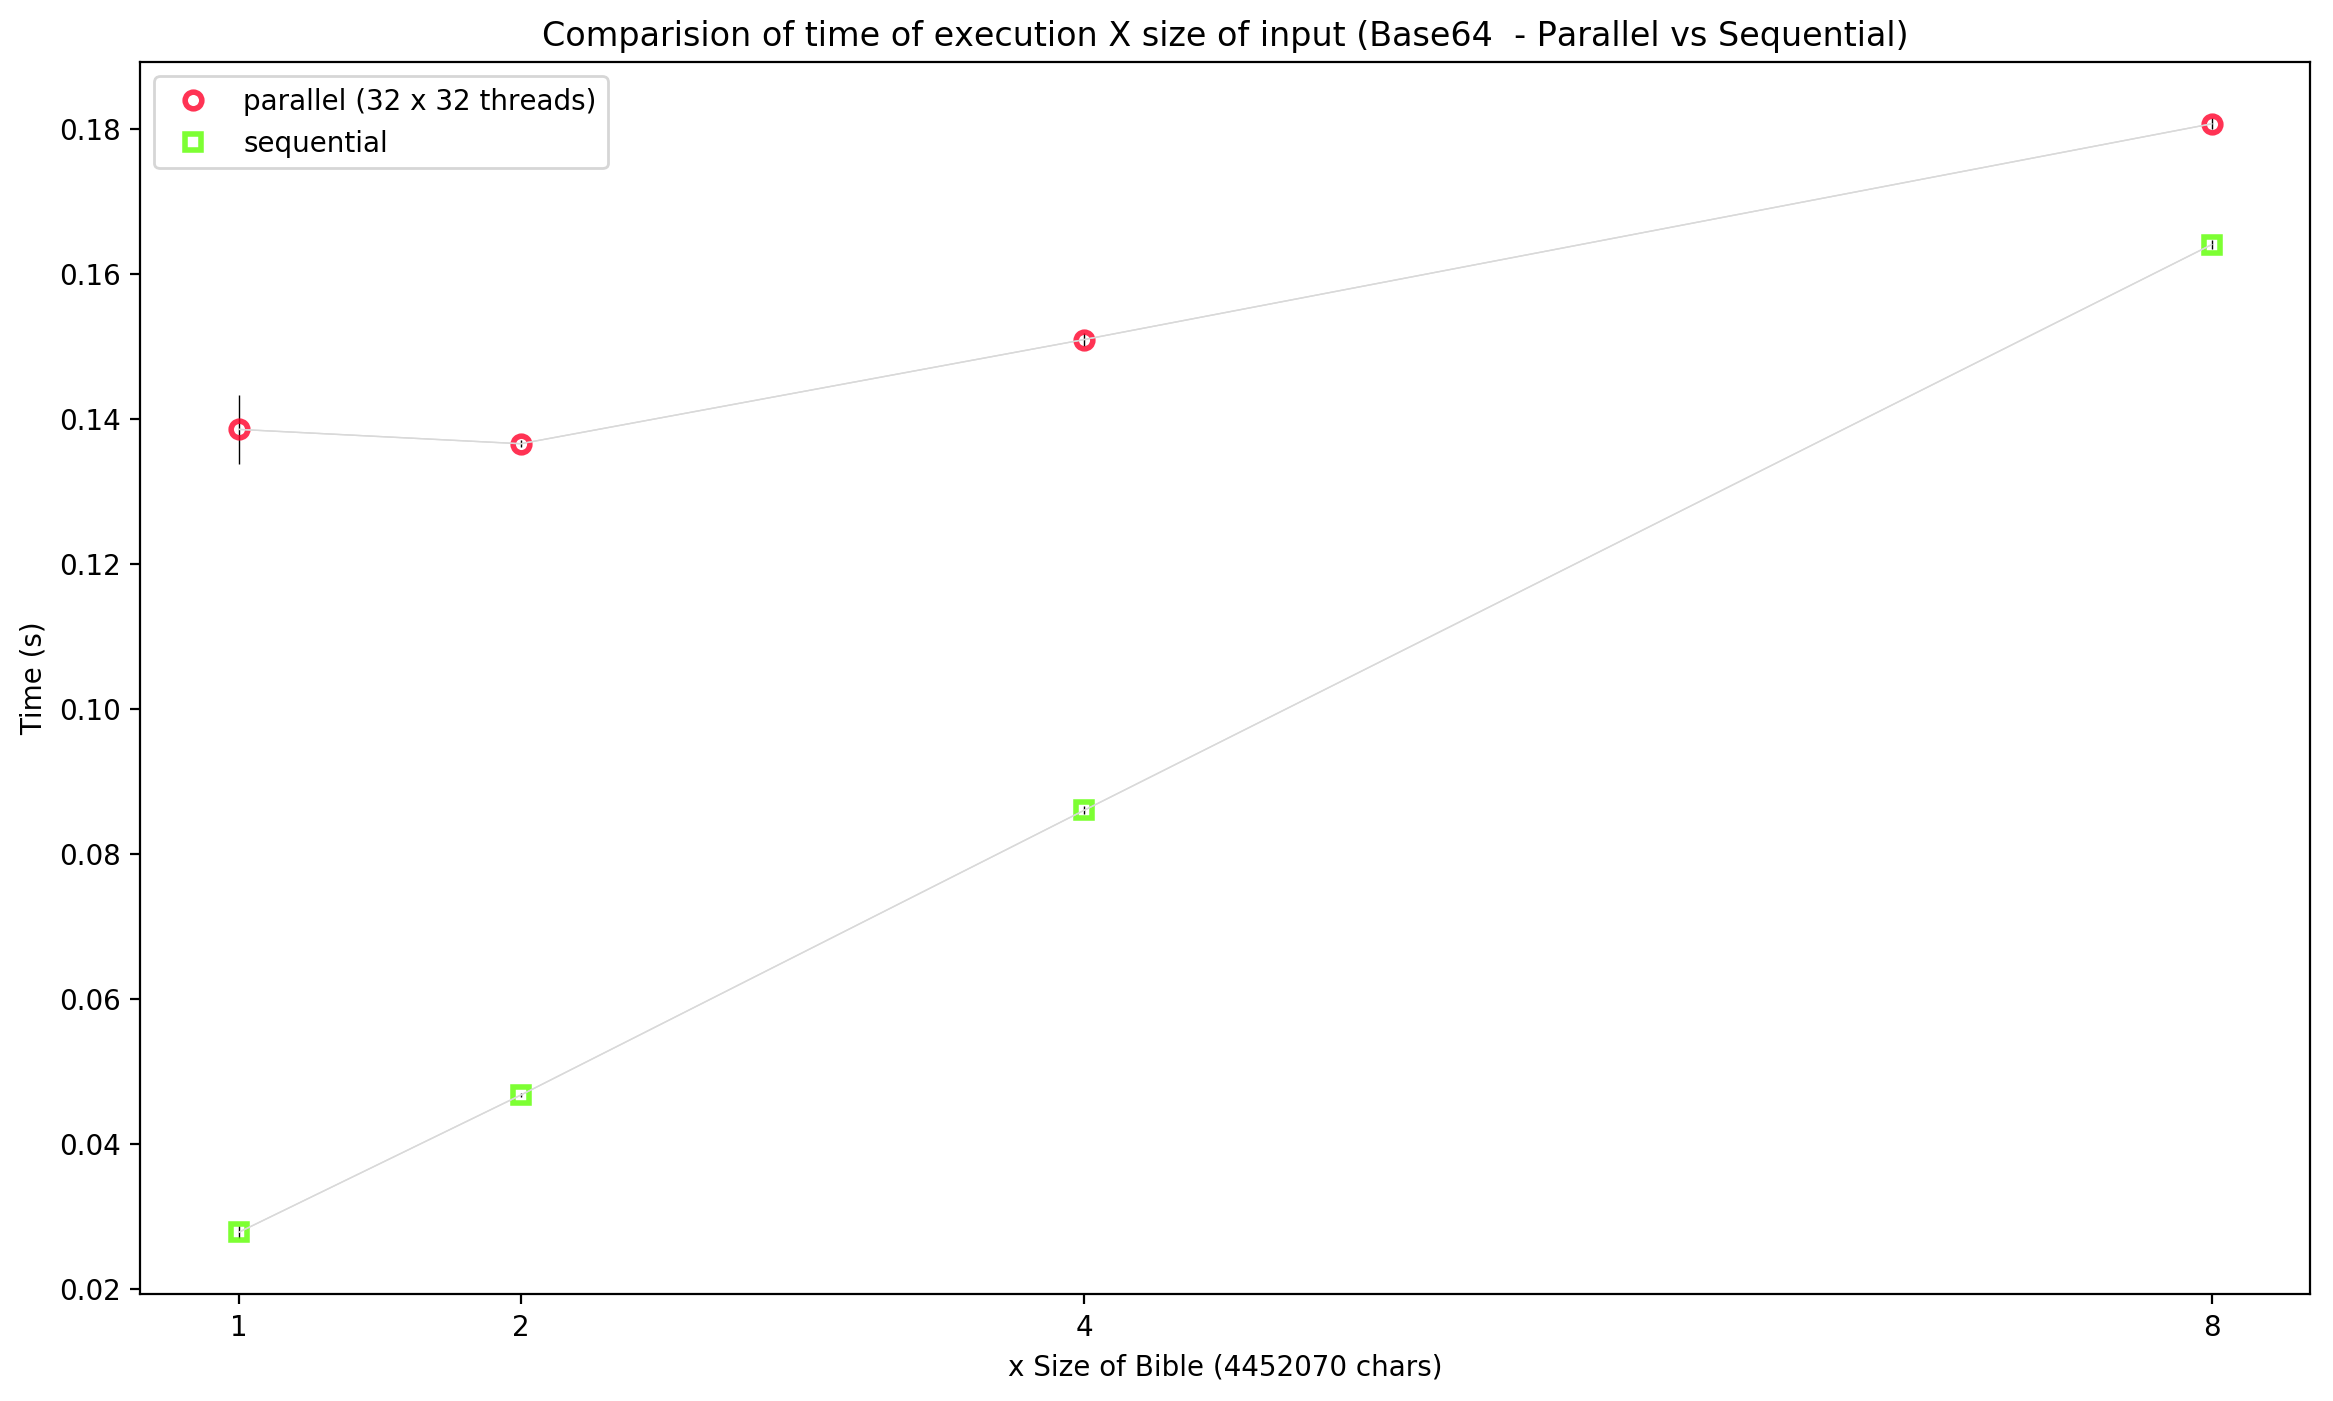
\includegraphics[scale=.4]{img/base64/parallelxseq.png}}
    \caption{Comparação entre implementações sequenciais e paralelas de
        Base64. Apesar do algoritmo sequencial ser mais rápido, é 
        possível notar que a versão paralela escala melhor no tamanho da
        instância, sugerindo que, para biblias maiores, o overhead de
        paralelismo seja compensado, tornando a implementação paralela
        a mais rápida.}
    \label{fig:base64_parallelseq}
\end{figure}

\begin{figure}[H]
    \makebox[\textwidth][c]{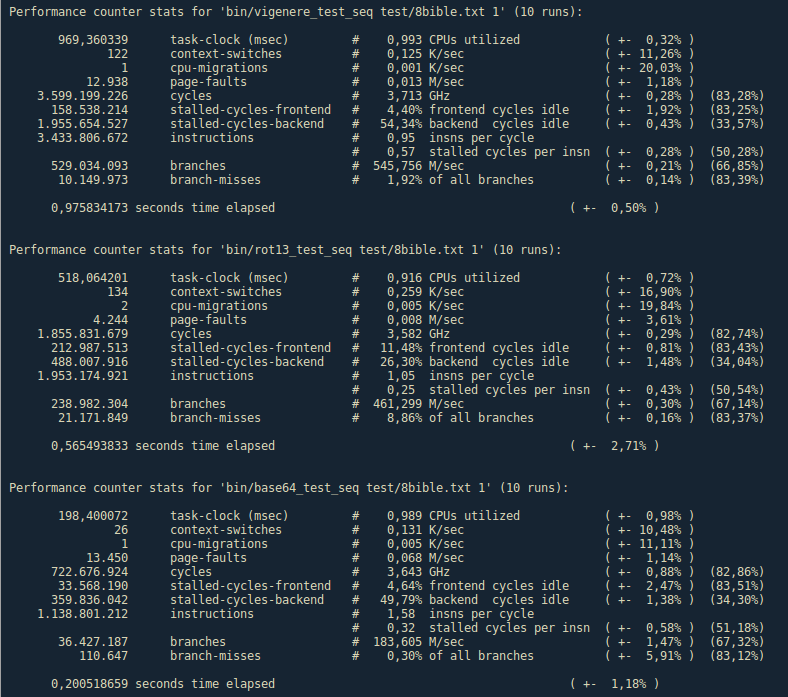
\includegraphics[scale=.4]{seq_perf.png}}
    \caption{Log do programa perf quando rodamos os três algoritmos 
    sequenciais implementados. É possível ver que o algoritmo Base64 é 
    rápido, fazendo com que o paralelismo só seja vantajoso com 
    instâncias maiores, quando comparamos com Vigenere e Rot13.}
    \label{fig:base64_seq_perf}
\end{figure}




%%%%%%%%%%%%%%%%%%%%% CONCLUSAO %%%%%%%%%%%%%%%%%%%%%%%%%%%%%%%%%%%%%%%%
\newpage
\section{Conclusão}
A partir dos dados analisados, podemos concluir que de fato a implementação paralela dos algoritmos mostrou ser mais rápida que a sequencial. Além disso também conseguimos notar o prejuízo das operações de leitura no algoritmo paralelo. Sem elas teríamos tempo constante para qualquer tamanho de entrada de arquivo (respeitando-se os limites máximos de threads por bloco e blocos por GPU).

Apesar dos resultados positivos, a princípio não esperavamos que o algoritmo paralelo só seria mais eficiente para tamanhos de entrada tão grandes. No entanto devemos lembrar que para os 3 algoritmos utilizados, o kernel mandado para a GPU é bastante simples. Caso tivessemos que fazer operações mais complexas para cada elemento do arquivo de entrada, talvez o algoritmo paralelo se tornaria mais rápido que o sequencial para um menor tamanho do arquivo de entrada. Nesse caso o ângulo da reta do \emph{tempo X tamanho de entrada} da implementação sequencial provavelmente aumentaria. Enquanto para o caso paralelo o ângulo seria mantido e um valor pequeno seria adicionado a cada ponto da reta. Isto é, supondo que as retas fossem dadas por $f(x) = ax + b$, para o caso sequencial $a$ aumentaria enquanto no paralelo $b$ aumentaria. Portanto concluímos que para utilizar o uso da GPU para algum programa que não tenha um tamanho de entrada tão grande só é vantajoso quando a complexidade da operação em cada elemento é suficientemente alta.


\end{document}
